\def\us{\char`\_}

\documentclass[a4paper, 12pt]{article}
%\documentclass{article}

\usepackage{fullpage}
\usepackage{pgf}
\usepackage{tikz}
\usetikzlibrary{arrows,automata,shapes}
\usepackage{multirow}
\usepackage{color}
\usepackage[latin1]{inputenc}
\usepackage{verbatim}
\usepackage{amsmath}
\usepackage{times,mathptmx}
\usepackage{chngcntr}
\usepackage{hyperref}
%\usepackage{draftwatermark}

\usepackage{listings}
\usepackage{cancel}
\graphicspath{ {../../figures/} }

%%%%%%%%%%%%%%%%%%%%%%%%%%%%%%%%%%%%%%%%%%%%%%%%%%%%%%%%%%%%%%%%%%%%%%%%%%%
% creating subsubsubsection notation
% src: http://www.latex-community.org/forum/viewtopic.php?f=5&t=791
%%%%%%%%%%%%%%%%%%%%%%%%%%%%%%%%%%%%%%%%%%%%%%%%%%%%%%%%%%%%%%%%%%%%%%%%%%%
\setcounter{secnumdepth}{6}
\renewcommand\theparagraph{\Alph{paragraph}}

\makeatletter
\renewcommand\paragraph{\@startsection{paragraph}{4}{\z@}%
                                     {-3.25ex\@plus -1ex \@minus -.2ex}%
                                     {0.0001pt \@plus .2ex}%
                                     {\normalfont\normalsize\bfseries}}
\renewcommand\subparagraph{\@startsection{subparagraph}{5}{\z@}%
                                     {-3.25ex\@plus -1ex \@minus -.2ex}%
                                     {0.0001pt \@plus .2ex}%
                                     {\normalfont\normalsize\bfseries}}
\counterwithin{paragraph}{subsubsection}
\counterwithin{subparagraph}{paragraph}
\makeatother
%%%%%%%%%%%%%%%%%%%%%%%%%%%%%%%%%%%%%%%%%%%%%%%%%%%%%%%%%%%%%%%%%%%%%%%%%%%%%%%%

\newcommand{\eqoffset}[1]{%
  {\ensuremath{%
      {\text{offset}}_{#1}}%
  }%
}
\newcommand{\eqdelay}[1]{{\text{delay}}_{#1}}
\newcommand{\eqasymm}{{\text{asymmetry}}}

\begin{document}

\title{White Rabbit calibration procedure\\[0.5cm]
\large {version 1.0}}
\author{Grzegorz Daniluk\\ CERN BE-CO-HT}

\maketitle
\thispagestyle{empty}

\begin{figure}[ht!]
  \centering
  \vspace{1.3cm}
  
\includegraphics[width=0.50\textwidth]{logo/WRlogo.pdf}
  \label{fig:wr_logo}
\end{figure}

\newpage

\newpage

\newpage

\tableofcontents

\newpage
\section{Introduction}

This document describes Wishbone configuration registers of the modules inside
the Gateware of the White Rabbit Switch. Each section gives a short description of
the module's role in the Switch design and is followed by a detailed description
of each configuration register available through Wishbone bus.


\newpage
\section{Definitions}
Before going further into the calibration procedure, some initial definitions
have to be clarified:

\begin{itemize}

	\item {\bf WR Device}: any device that supports White Rabbit
		synchronization over an optical link. This can be e.g. the White Rabbit
		Switch, the SPEC board, or any custom hardware made for a specific
		application. A WR Device can run as WR Master or/and WR Slave.

	\item {\bf WR Calibrator}: any White Rabbit Device selected from the 
		available set that is used as a reference to calibrate the 
		rest of the White Rabbit Devices used in a synchronization system.

	\item {\bf WR Device TX latency} ($\Delta_{TX}$): WR PTP packet delay 
		from the moment it is timestamped in the transmission circuit
		inside the FPGA (WR Endpoint module) to the moment when the 
		transmitted packet reaches a fiber link. It is the sum of: 
		transmission delay inside FPGA chip; propagation delay of 
		electronic components and PCB traces; SFP transmitter delay.

	\item {\bf WR Device RX latency} ($\Delta_{RX}$): WR PTP packet delay 
		from the moment it reaches the receiving SFP module, to the 
		moment it is timestamped in the reception circuit inside the FPGA (WR
		Endpoint module). It is the sum of: SFP receiver delay; 
		propagation delay of electronic components and PCB traces; 
		reception delay inside FPGA chip.

	\item {\bf WR Device asymmetry} (2$\beta$): the difference between the TX 
		latency $\Delta_{TX}$ and the RX latency $\Delta_{RX}$.

	\item {\bf Fiber round-trip latency} ($\delta$): the total round-trip 
		delay of a fiber link (without the Tx/Rx latencies of the WR Devices). 
		It is the sum of the one-way propagation delays: Master-to-Slave 
		($\delta_{MS}$) and Slave-to-Master ($\delta_{SM}$).

	\item {\bf Relative delay coefficient} ($\alpha$): the parameter describing 
		the asymmetry (the difference between $\delta_{MS}$ and 
		$\delta_{SM}$) of the fiber used in a White Rabbit network. It 
		is the relative difference of Master-to-Slave and Slave-to-Master 
		propagation delays ($\alpha = \frac{\delta_{MS} - \delta_{SM}}
		{\delta_{SM}}$).

	\item {\bf Round trip delay} ($delay_{MM}$): the total packet delay on 
		a White Rabbit link. It is the sum of communicating parties (Master and
		Slave) fixed delays ($\Delta_{TXM}$, $\Delta_{RXM}$, $\Delta_{TXS}$,
		$\Delta_{RXS}$), bitslide values ($\epsilon_M$,
    $\epsilon_S$) and fiber round-trip latency ($\delta$).

\end{itemize}


\newpage
\section{Equipment requirements}

The calibration procedure described in this document makes no assumption on what 
kind of WR device will be used as a WR Calibrator or what kind of fiber (length, 
producer) is placed in between WR Devices. However, there are a few general 
requirements listed below. The first two of them are essential for the
Calibrator pre-calibration steps described in section
\ref{sec:procedure:calibrator}.\\

WR Calibration needs:
\begin{itemize}
	\item two fiber cables having different lengths, one of them is a few
		kilometers long (to make $\alpha$ coefficient measurement precise), while
		the other is a few meters long.
	\item two pieces of a WR Device selected to be the Calibrators: this means two
		exactly the same WR Devices, having the same PCB design, the same bitstream
		downloaded into the FPGA and using complementary SFP transceivers (the same
		producer, matching Tx/Rx WDM wavelengths\footnote{Check the list of
		supported SFP transceivers http://www.ohwr.org/projects/white-rabbit/wiki/SFP});
	\item all WR Devices (i.e. the Calibrator and devices under calibration)
		capable of producing 1-PPS output from their local clock 
		and providing it through an on-board connector or test point;
	\item two oscilloscope cables of the same delay (i.e. the same type and
		length) or different but known delays so that the correction
		could be made for all oscilloscope measurements described in
		the document;
	\item a device of any producer that is able to measure time
		spans of less than 1ns for measuring 1-PPS skew. This can be an oscilloscope or timer/counter device e.g. Pendulum CNT-91.
\end{itemize}


\newpage
\section{Calibration procedures}
\label{sec:calib_proc}
\subsection{Initial state}
Initially none of the transmission/reception latencies and asymmetry of White 
Rabbit devices or fiber parameters are known. Therefore {\bf the values of 
appropriate parameters should be set to 0 for all nodes and switches which will
be calibrated}. In the White Rabbit PTP Core this can be done by modifying the SFP
database and setting $\Delta_{TX}$, $\Delta_{RX}$ and $\alpha$ values to 0 for all
supported transceivers\footnote{Please refer to the White Rabbit PTP Core manual
\url{http://www.ohwr.org/projects/wr-cores/documents}}. For the White Rabbit Switch 
please modify the \emph{/wr/etc/sfp\_database.conf} and
\emph{/wr/etc/wrsw\_hal.conf} configuration files.

\subsection{Reference fiber latency}
\label{subsec:refiber}

In this very first step of the calibration procedure the total propagation delay
($\delta = \delta_{MS} + \delta_{SM}$) of a fiber cable is measured. It requires
two different fiber cables with LC connectors (i.e. fibers that have
different length). For further considerations let's mark them $f_1$ and $f_2$.
Fiber $f_1$ can be called helper and is just a few meters long. It is used to
measure the parameters of $f_2$ and in hardware calibration procedures described
later. Fiber $f_2$ is of the same type that will be used in the WR installation.
It is a few kilometers long and its parameters will be measured.

\begin{figure}[ht]
	\begin{center}
		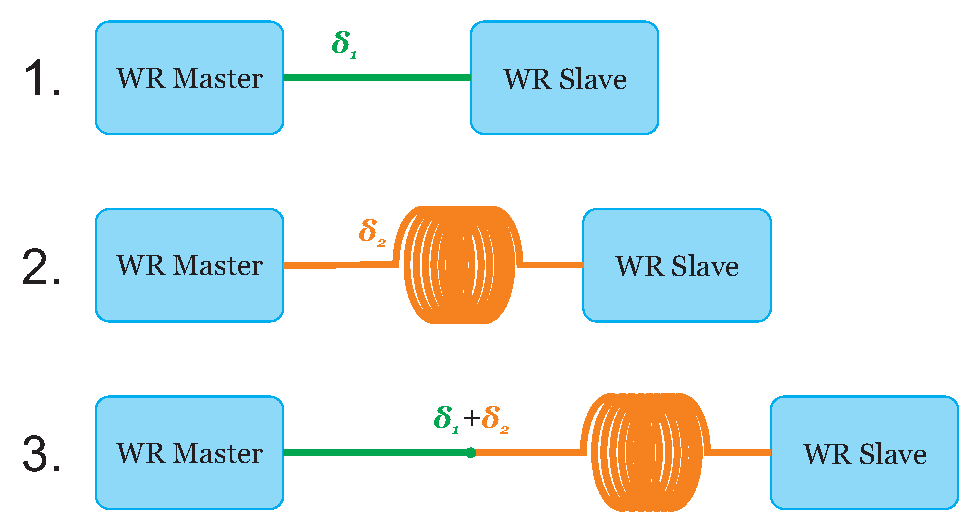
\includegraphics[width=.6\textwidth]{calibration/fiber_1.pdf}
		\caption{Measuring total fiber propagation latency}
		\label{fig:refiber:latency}
	\end{center}
\end{figure}

\begin{enumerate}
	\item Take two White Rabbit devices, configure one of them as WR Master 
		and the other as WR Slave. 
	\item Connect them with fiber $f_1$ and wait until they become 
		synchronized (fig.\ref{fig:refiber:latency}, step 1). You can 
		use the available monitoring software \footnote{\emph{gui} WRPC 
		Shell command for the WR PTP Core, or \emph{wr\_mon} program for the WR 
		Switch} on the Slave device to check when it happens (indicated by 
		the WR servo in the \emph{TRACK\_PHASE} state and an offset below 1 ns).
	\item Write down the round trip delay ($delay_{MM1}$) reported by
		the monitoring software and the bitslide values for both
		Master($\epsilon_{M1}$) and Slave($\epsilon_{S1}$). Since the fixed delays
    are initially set to 0, the bitslide values are reported by the monitoring
		software simply as the reception delays.
	\item Connect the same two WR Devices with fiber $f_2$
		(fig.\ref{fig:refiber:latency}, step 2), wait again until the WR Slave
		becomes synchronized and write down the values of
		$delay_{MM2}$, $\epsilon_{M2}$ and $\epsilon_{S2}$.
	\item Connect fibers $f_1$ and $f_2$ together using an LC-LC Adapter and use
		this link to connect again the same WR Devices together(fig.
		\ref{fig:refiber:latency}, step 3). Wait until the WR Slave becomes 
		synchronized and write down the values of $delay_{MM3}$, 
		$\epsilon_{M3}$, $\epsilon_{S3}$.
	\item Subtract the bitslide values to obtain an approximation of the round
		trip delay, the sum of Master and Slave latencies ($\Delta_{TXM}$,
		$\Delta_{RXM}$, $\Delta_{TXS}$, $\Delta_{RXS}$) and the fiber round-trip
		latency:
		\begin{align}
			\label{equ:refiber:delmmeps1}
			delay_{MM1}' = delay_{MM1} - \epsilon_{M1} -
			\epsilon_{S1} \\
			\label{equ:refiber:delmmeps2}
			delay_{MM2}' = delay_{MM2} - \epsilon_{M2} -
			\epsilon_{S2} \\
			\label{equ:refiber:delmmeps3}
			delay_{MM3}' = delay_{MM3} - \epsilon_{M3} -
			\epsilon_{S3}
		\end{align}
	\item Calculate the latency of the fiber $f_1$ ($\delta_1$) and $f_2$
		($\delta_2$):
		\begin{align}
			\delta_1 = delay_{MM3}' - delay_{MM2}' \\
			\delta_2 = delay_{MM3}' - delay_{MM1}'
		\end{align}
		{\bf Note:} The LC-LC Adapter also has its own unknown latency that
		introduces an error in the $\delta_1$ and $\delta_2$ calculations.
		However, this error is a few picoseconds and can be disregarded.
\end{enumerate}
Further mathematical explanation for this calibration step can be found in
appendix \ref{subsec:app_filat}. Fiber cable $f_1$ with a round-trip latency
$\delta_1$ will be used further to pre-calibrate the selected WR Calibrator.

\subsection{Fiber asymmetry}
\label{subsec:fiasym}

The calibration of a fiber cable is needed to find out its asymmetry coefficient
$\alpha$. In the previous step we managed to calculate the total propagation
latency of fibers $f_1$ and $f_2$. However, to calibrate any device, the fiber
asymmetry has to be known.

The $\alpha$ coefficient used in the White Rabbit protocol to express fiber 
asymmetry is defined as:
\begin{equation}
	\alpha = \frac{\delta_{MS} - \delta_{SM}}{\delta_{SM}}
\end{equation}

To get its value, you have to make two connections with WR Devices and fibers
$f_1$, $f_2$ as presented in figure \ref{fig:fiasym}.

\begin{figure}[ht]
	\begin{center}
		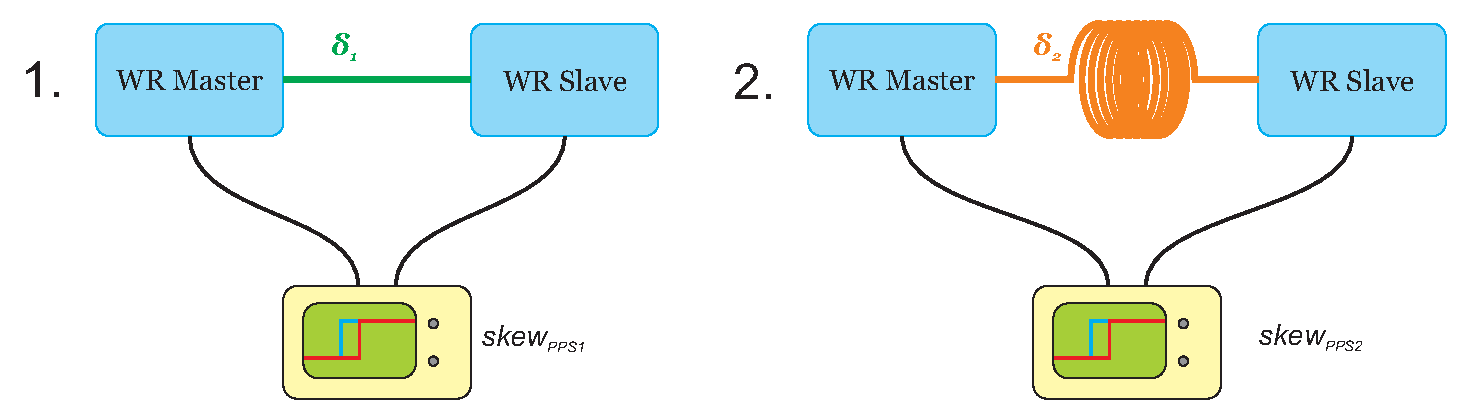
\includegraphics[width=.9\textwidth]{calibration/fiber_2.pdf}
		\caption{Measuring fiber $f_2$ asymmetry}
		\label{fig:fiasym}
	\end{center}
\end{figure}

\begin{enumerate}
	\item Connect any two WR Devices with a few meters long fiber $f_1$, set
		the $\alpha$ value in their configuration to 0, configure one of them as WR
		Master, and the other as WR Slave. Connect their 1-PPS outputs to an
		oscilloscope. 
		
		It is important to use oscilloscope cables of the same length
		and type or cables with known delays so that no additional,
		unknown latency affects the measurements.

	\item Use the monitoring software to check when the Slave becomes
		synchronized to the Master (offset reported by WR PTP daemon below 
		1 ns and WR servo in the \emph{TRACK\_PHASE} state).

	\item Measure 1-PPS skew between the Slave and Master in picoseconds by
		comparing the 1-PPS signals with an oscilloscope ($skew_{PPS1} 
		= t_{PPS_S} - t_{PPS_M}$)

	\item Repeat the same procedure using a few kilometers long fiber $f_2$ to
		obtain the PPS skew for the second connection ($skew_{PPS2} =
		t_{PPS_S}' - t_{PPS_M}'$)

	\item Calculate the $\alpha$ coefficient using the following equation:
		\begin{equation}
			\alpha = \frac{2(skew_{PPS2} -
			skew_{PPS1})}{\frac{1}{2}\delta_2 -
			(skew_{PPS2}-skew_{PPS1})}
		\end{equation}

  \item The White Rabbit Switch uses the $\alpha$ value calculated from the equation
    above without any conversion. However, the White Rabbit PTP Core requires
    converting $\alpha$ into a natural number using the formula:
    \begin{equation}
      \alpha_N = 2^{40}(\frac{\alpha+1}{\alpha+2} - 0.5)
    \end{equation}

  \item $\alpha$ or $\alpha_N$ (depending on the WR Device) should be stored
		into the configuration parameters of a WR Calibrator but also into
		each Slave device that will use this fiber.
\end{enumerate}

Further mathematical explanation for this calibration step can be found in
appendix \ref{subsec:app_fiasym}

{\bf Note:} Both WR Devices used at CERN: the WR Switch and the WR PTP Core can
be used to calculate the $\alpha$ value. However, the 1-PPS signal generated by
the WR PTP Core running on the SPEC card with a DIO mezzanine is more jittery
than the 1-PPS generated by the WR Switch (check measurement uncertainty
considerations in appendix \ref{subsec:errors:fiasym}). For most applications
the inaccuracy of $\alpha$ measured using two SPEC cards will be negligible. If
that isn't the case, the most precise value of the $\alpha$ parameter can be
obtained from the measurements described above done with two WR Switches.
Alternatively, measurements done with two SPEC cards (or any other hardware
based on the SPEC design) can be repeated multiple times to produce an averaged
value of 1-PPS skew and a more accurate $\alpha$.


\subsection{Calibrator pre-calibration}
\label{sec:procedure:calibrator}

Having the parameters of fiber $f_1$ measured, a WR Calibrator has to be
selected among the set of available WR-compatible devices. The only
constraint for the selection is having two instances of the same device
for the pre-calibration procedure described here. They must have the
same PCB layout and the same FPGA bitstream.

To determine what are the transmission and reception latencies ($\Delta_{TX}$,
$\Delta_{RX}$) of the WR Calibrator, the connection shown in figure
\ref{fig:calibrator} has to be established.

\begin{figure}[ht]
	\begin{center}
		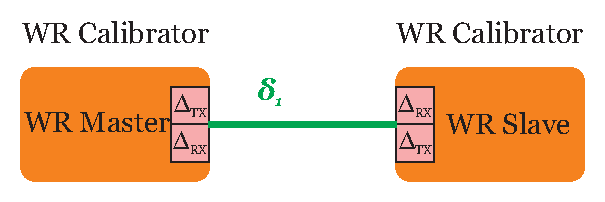
\includegraphics[width=.5\textwidth]{calibration/calibrator.pdf}
		\caption{Measuring Calibrator latencies}
		\label{fig:calibrator}
	\end{center}
\end{figure}

\begin{enumerate}
	\item Since both Master and Slave are exactly the same devices (the same FPGA
		bitstreams, PCB layout, complementary SFPs from the same producer) the sum
		of their TX and RX latencies is equal:
		\begin{equation} 
			\Delta_{TXM} + \Delta_{RXM} = \Delta_{TXS} + \Delta_{RXS} 
		\end{equation}
		That means, the total transmission delay caused by each of those devices can
		be determined by simply dividing by 2 the round trip delay without the RX
		bitslide of each device and the fiber round-trip latency:
		\begin{equation}
			\Delta_{TX} + \Delta_{RX} = (delay_{MM1}' - \delta_1) /
			2
		\end{equation}
	\item Naturally, our Calibrator has some internal asymmetry, which means that
		$\Delta_{TX} \neq \Delta_{RX}$. There are two ways to determine the exact
		values of $\Delta_{TX}$ and $\Delta_{RX}$. It can be done either by
		establishing a WR link with a WR Device having a well-known internal
		asymmetry - which we don't have since all other devices will be calibrated
		from the WR Calibrator; or taking apart the Calibrator and measuring the
		latency of PCB traces, electronic components, SFP transceivers - that is
		possible, not trivial at all, and raises many other problems like measuring
		the latency between the SFP electrical input and its optical output, or
		measuring the latency inside the FPGA chip. Therefore at this point we set
		up a convention, that the WR Calibrator has no asymmetry:
		\begin{equation}
			\Delta_{TX} = \Delta_{RX}
		\end{equation}
		That means, the parameters describing the transmission and reception delays
		of the WR Calibrator should be set in the device configuration to:
		\begin{equation}
			\Delta_{TX} = \Delta_{RX} = (delay_{MM1}' - \delta_1) /
			4
		\end{equation}

		{\bf Note:} Don't worry, assuming that the WR Calibrator has no asymmetry
    does not affect the calibration quality. It is taken into account later
    during the actual calibration of each unknown WR Device. It also does not
    affect the WR PTP protocol when a link is established between two WR
    Calibrators, since the daemon only uses the precise value of the one-way,
    Master to Slave link delay (where the TX latency of the Master and RX
    latency of the Slave are summed together).
		
	\item Configure your WR Calibrator with the calculated $\Delta_{TX}$ and
		$\Delta_{RX}$ values - modify the SFP database for the WR PTP Core, or the
		\emph{/wr/etc/wrsw\_hal.conf} file for the WR Switch.
\end{enumerate}


\subsection{WR Device calibration} 
\label{subsec:devices}

Having the WR Calibrator selected among the available WR Devices, and the fiber
cable used in the previous steps (with known $\alpha$ coefficient and total
propagation delay $\delta$), you can start calibrating all other devices that
will later create a White Rabbit Network (fig.\ref{fig:devices}). 

\begin{figure}[ht]
	\begin{center}
		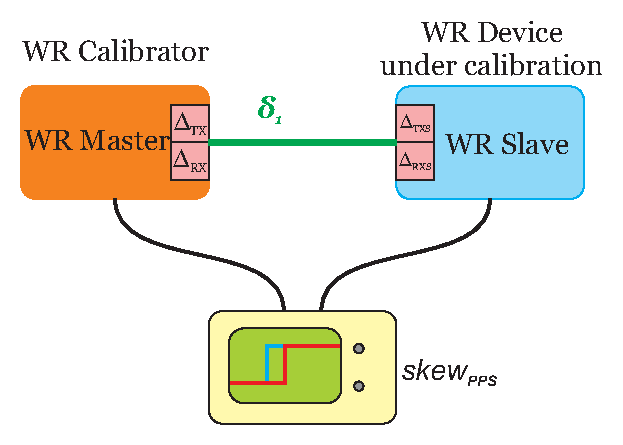
\includegraphics[width=.5\textwidth]{calibration/wr_device.pdf}
		\caption{WR Device calibration with WR Calibrator and known
		fiber $f_1$}
		\label{fig:devices}
	\end{center}
\end{figure}

\begin{enumerate}
	\item Connect your Calibrator to an unknown WR Device using the fiber with the
		known $\alpha$ measured earlier (\ref{subsec:fiasym}). Remember to use an
		appropriate SFP transceiver on each side depending on whether your device
		under calibration is supposed to run as a WR Master or a WR
		Slave\footnote{There is a wiki page describing which wavelength should be
		used on each side: \url{http://www.ohwr.org/projects/white-rabbit/wiki/SFP}}.
		If you want to have the flexibility of selecting Master/Slave mode later
		through device configuration, the calibration procedure described below
		should be performed twice - with the SFP that will be used in Master, and
		the SFP that will be used in Slave mode. In further steps of this procedure
		the assumption is made that the WR Device being calibrated runs in WR Slave
		mode.
	\item Run the monitoring software on the Slave node and write down the
		round-trip delay ($delay_{MM}$) and fixed delays of both Master and Slave
		($\Delta_{TXM}$, $\Delta_{RXM}$, $\Delta_{TXS}$, $\Delta_{RXS}$). The
		transmission delay for Slave is reported to be 0, while the reception delay
		may be non-zero. It is the current RX bitslide value $\epsilon_S$.
	\item Calculate the average (coarse) transmission and reception delays for the
		Slave device:
		\begin{equation}
			\label{equ:devices:coarsedtxrx}
			\Delta_{TXS}' = \Delta_{RXS}' = \frac{1}{2} \Delta_S = 
			\frac{1}{2}(delay_{MM} - \Delta_{TXM} - \Delta_{RXM} - 
			\epsilon_S - \delta_1)
		\end{equation}
	\item Write the $\Delta_{TXS}$ and $\Delta_{RXS}$ delays to the configuration
		of your device, and restart its PTP daemon so that it synchronizes again
		using the new values.
	\item At this point your WR Device knows the coarse values of the transmission
		and reception delays. You can connect the 1-PPS signals generated by the
		calibrator and the device to an oscilloscope to observe that there is still
		some offset of (probably) a few nanoseconds between the Slave and Master
		even if the PTP daemon reports it is close to 0. That is because the
		transmission and reception delays are not equal (as the coarse values
		above). This asymmetry has to be measured and used to correct the coarse
		values of $\Delta_{TXS}$ and $\Delta_{RXS}$.
	\item Measure the Slave to Master offset by comparing the 1-PPS skew with the
		oscilloscope. This is the correction value that has to be subtracted from
		the coarse $\Delta_{TX}$ and added to $\Delta_{RX}$ to compensate the
		hardware asymmetry:
		\begin{align}
			\Delta_{TXS} = \frac{1}{2}\Delta_S - skew_{PPS} \\
			\Delta_{RXS} = \frac{1}{2}\Delta_S + skew_{PPS}
		\end{align}

		{\bf Note:} The asymmetry measured in this stage of calibration is in fact
		the sum of WR Device and WR Calibrator asymmetry. However, since both
		transmission and reception delays are modified with this value, the
		component for WR Calibrator asymmetry will cancel when connecting two WR
		Devices calibrated to the same Calibrator, see \ref{subsec:apx:devices} for
		a mathematical proof.
	\item After putting the new delay values in the configuration of the WR
		Device, the PTP daemon can be restarted and this time the device will
		synchronize to the Calibrator with an offset below 1ns.
	\item This procedure has to be repeated for all other WR Devices (WR Masters
		and WR Slaves). When you want to calibrate a WR Switch, this calibration
		procedure has to be performed for each WR port of the device.
\end{enumerate}


\newpage
\section{Measuring already deployed fiber}

Most of the methods described in section \ref{sec:calib_proc} require making a
measurement of 1-PPS signals produced by WR Devices. It's fairly easy to compare
them when you have a roll of fiber and the devices being calibrated lying on a
desk in the laboratory. However, sometimes the fiber infrastructure which
will be used in a WR network is already installed. WR Devices can still be
collected in a lab for calibration, but measuring the $\alpha$ parameter of a
buried fiber is not as straightforward as in section \ref{subsec:fiasym}. This
section proposes a way of measuring 1-PPS skew when the fiber cable is
already installed and you don't have both ends next to each other. The
measurements made this way can be used as a substitute for the simple
oscilloscope measurements in section \ref{sec:calib_proc}.

\subsection{Measurement with a loop-back fiber}
\label{subsec:loopback}
This method is based on a fiber delay calibration procedure used in the CERN
Neutrinos to Gran Sasso project \cite{cngs}. It requires:
\begin{itemize}
	\item an additional fiber which will be used to transmit the 1-PPS signal
		produced by a distant WR Device to the place where it can be compared
		locally with the other WR Device using an oscilloscope
	\item two oscilloscope cables of the same type - having equal latency or a
    known latency difference which can be taken into account and compensated
	\item one pair of optical transmitter and receiver which will be used to
		convert the 1-PPS electric signal into a light impulse sent through the
		loop-back fiber. The transmitter and receiver must have constant
		transmission/reception delays that don't vary on each power cycle.
\end{itemize}

\begin{figure}[ht]
	\begin{center}
	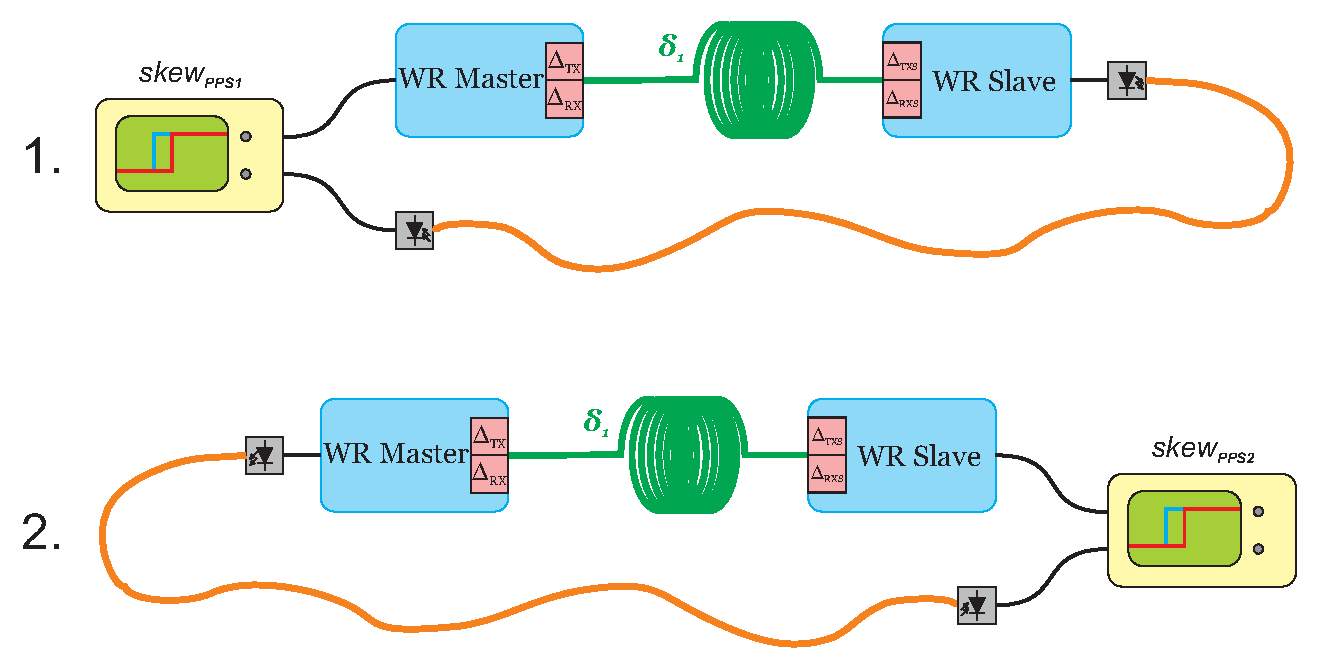
\includegraphics[width=.8\textwidth]{calibration/loopback_fibre.pdf}
	\caption{Measuring 1-PPS offset using a loop-back fiber}
	\label{fig:loopback}
	\end{center}
\end{figure}

Measurement procedure:
\begin{enumerate}
	\item When a link is established between the WR Master and the WR Slave,
		connect the optical transmitter to the 1-PPS signal produced by the WR Slave
		and the loop-back fiber. On the other side of the fiber connect the optical
		receiver (fig.\ref{fig:loopback}, step 1).
	\item Measure the 1-PPS skew ($skew_{PPS1}$) between the Slave (1-PPS
		transmitted through the loop-back fiber) and the Master (1-PPS directly from
		the node) using an oscilloscope.
	\item Swap the optical transmitter and receiver so that you'll now transfer
		the 1-PPS signal generated from the WR Master using the same loop-back fiber
		to the WR Slave side (fig.\ref{fig:loopback}, step 2).
	\item Do the same 1-PPS skew measurement between the Slave and Master, but
		this time on the WR Slave side (the 1-PPS comes directly from the WR Slave
		node and the one from the WR Master is transmitted through the loop-back
		fiber). This way you will obtain the value $skew_{PPS2}$.
	\item Calculate the actual skew between the WR Master and WR Slave using the
		equation:
	\begin{equation}
	skew_{PPS} = \frac{1}{2} (skew_{PPS1} + skew_{PPS2})
	\end{equation}
\end{enumerate}

The skew value calculated that way can be used in any equation from section
\ref{sec:calib_proc}. However, please remember that you will also need the
latency of the fiber ($\delta_1$ in figure \ref{fig:loopback}). That means, you
would have to start the calibration with two WR Devices on your desk, connected
with a short (few meters long) link (procedure \ref{subsec:refiber}) and later
use these two WR Devices with the already-installed link.


\newpage
\section{Recovering the calibrator}

In a real life, when a WR network operates for a few years, the WR Device selected
to be a calibrator might become broken. The lack of a WR Calibrator makes it
impossible to connect new devices without recalibrating the whole WR network.
This section presents a method for obtaining the $\Delta_{TX}$, $\Delta_{RX}$
delays for a WR Device so that it can be used as the new WR Calibrator for an
already-deployed network.

\begin{figure}[ht]
	\begin{center}
	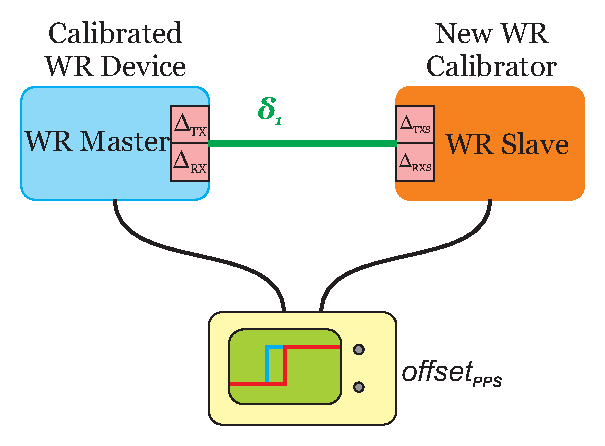
\includegraphics[width=.5\textwidth]{calibration/recover_calibrator.ps}
	\caption{Calibrating a new WR Calibrator for an already-existing WR network}
	\label{fig:recover_calibrator}
	\end{center}
\end{figure}

\begin{enumerate}
	\item Initially please set the transmission and reception delays
		($\Delta_{TXS}$, $\Delta_{RXS}$) of the new WR Calibrator to 0, but $\alpha$ has
		to be set to the correct value for fiber $f_1$.
	\item Connect your new WR Calibrator to one of the WR Devices originally
		calibrated to the primary WR Calibrator
		(fig.\ref{fig:recover_calibrator}). Use a short (few meters) fiber of known
		latency and $\alpha$ coefficient or measure it first according to the
		instructions in sections \ref{subsec:refiber} and \ref{subsec:fiasym}. Set
		the WR Calibrator to Slave, and the WR Device to Master mode.
	\item Run the monitoring software on the Slave node (\emph{wr\_mon} for the WR
		Switch or \emph{gui} for the WR PTP Core). Write down the round-trip
		delay and fixed delays of both Master and Slave. The transmission delay of
		the Slave ($\Delta_{TXS}$) should be 0, but its reception delay
		($\Delta_{RXS}$) will be equal to the RX bitslide value $\epsilon_S$. The
		reception delay of the Master ($\Delta_{RXM}$) already includes the bitslide
		value for this device.
	\item Calculate the average (coarse) transmission and reception delay for the
		new Calibrator using the values read from the monitoring software and the
		latency of the fiber ($\delta_1$):
	\begin{equation}
		\Delta'_{TXS} = \Delta'_{RXS} = \frac{1}{2}\Delta_S = \frac{1}{2}(delay_{MM} - \Delta_{TXM} - \Delta_{RXM} - \Delta_{RXS} - \delta_1)
	\end{equation}
	\item Write the $\Delta_{TXS}$ and $\Delta_{RXS}$ delays to the configuration
		of the new WR Calibrator, restart the device, and let it synchronize again
		with the new values.
	\item Measure the Slave to Master offset by comparing 1-PPS signals with an
    oscilloscope. The 1-PPS skew ($skew_{PPS}$) is used as
    a correction value for the coarse transmission/reception delays:
	\begin{align}
		\Delta_{TXS} = \frac{1}{2}\Delta_S - skew_{PPS}\\
		\Delta_{RXS} = \frac{1}{2}\Delta_S + skew_{PPS}
	\end{align}
	\item Update the configuration of the new WR Calibrator to replace the coarse
		delays with $\Delta_{TXS}$, $\Delta_{RXS}$.
	\item The new WR Calibrator can be used to calibrate any other WR Device that is
		supposed to be connected to the existing WR network.\\[12pt]
	{\bf Note:} Please be aware that the measurement errors accumulate. It might
	become an issue if the new calibrator uses values recovered with a WR Device
	that was already calibrated to a recovered calibrator. The longer this chain
	is, the more inaccuracy you should expect from the calibration procedure. To
	minimize this effect, it's better to recover the values for the new WR
	Calibrator using only devices that were calibrated to the primary WR
	Calibrator for a given network.
\end{enumerate}


\appendix
\newpage
\section{Mathematical proofs}

\subsection{Reference fiber latency}
\label{subsec:app_filat}
The same pair of WR Devices is used for all three connections in this procedure.
That is why, when considering round-trip delay after subtracting the bitslide
values, the transmission and reception delays of both devices are summed
together and remain constant for fiber $f_1$, $f_2$, $f_1 + f_2$:
\begin{equation}
	\Delta = \Delta_{TXM} + \Delta_{RXM} + \Delta_{TXS} + \Delta_{RXS}
\end{equation}

When two fibers $f_1$, $f_2$ are joined together the fiber latency for this
connection will be the sum of $\delta_1$ and $\delta_2$. After eliminating the 
bitslide value, the remaining part of a round trip delay consists of the 
following elements:
\begin{equation}
	delay_{MM1}' = \Delta + \delta_1\\
\end{equation}
\begin{equation}
	delay_{MM2}' = \Delta + \delta_2\\
\end{equation}
\begin{equation}
	delay_{MM3}' = \Delta + \delta_1 + \delta_2
\end{equation}

This equation system has three unknowns and after solving gives the formulas for
the round-trip fiber latencies:
\begin{align}
	\delta_1 = delay_{MM3}' - delay_{MM2}'\\
	\delta_2 = delay_{MM3}' - delay_{MM1}'
\end{align}

\subsection{Fiber asymmetry}
\label{subsec:app_fiasym}

In this step of the calibration procedure two WR connections with the same pair
of devices are established. For each of them the offset between the WR Slave and
WR Master is calculated by the WR PTP software as:
\begin{equation}
	offset_{MS} = t_1 - t_2 + delay_{MS}
\end{equation}

\noindent where $delay_{MS}$ is an estimated one-way link delay. When $\alpha$ is
initially equal to 0, $delay_{MS}$ is estimated as half of the round-trip
delay, which results in a distorted offset between the two devices:
\begin{equation}
	offset_{MS}' = t_1 - t_2 + \frac{1}{2} delay_{MM}
\end{equation}

\noindent Then $skew_{PPS}$ measured with an oscilloscope is equal to the
uncompensated link asymmetry (the sum of the fiber asymmetry and hardware
asymmetry):
\begin{align}
  \label{equ:app_fiasym:skew1}
  skew_{PPS1} &= offset_{MS1} - offset'_{MS1} = delay_{MS1} - \frac{1}{2} delay_{MM1}\\
  \label{equ:app_fiasym:skew2}
  skew_{PPS2} &= offset_{MS2} - offset'_{MS2} = delay_{MS2} - \frac{1}{2} delay_{MM2}
\end{align}

\noindent We also know what factors build up the round trip delays and one-way
delays for both connections. Please notice since the same pair of the devices is
used in both cases, fixed hardware delays stay the same:
\begin{align}
  delay_{MM1} &= \Delta + \delta_1\\
  delay_{MM2} &= \Delta + \delta_2\\
  delay_{MS1} &= \Delta_{TXM} + \Delta_{RXS} + \delta_{MS1}\\
  delay_{MS2} &= \Delta_{TXM} + \Delta_{RXS} + \delta_{MS2}\\
     \delta_1 &= \delta_{MS1} + \delta_{SM1}\\
     \delta_2 &= \delta_{MS2} + \delta_{SM2}
\end{align}

\noindent Using the formulas above, equations \ref{equ:app_fiasym:skew1} and
\ref{equ:app_fiasym:skew2} can be expanded:
\begin{align}
  skew_{PPS1} &= \Delta_{TXM} + \Delta_{RXS} + \delta_{MS1} - \frac{1}{2}\Delta
  - \frac{1}{2} \delta_1\\
  skew_{PPS2} &= \Delta_{TXM} + \Delta_{RXS} + \delta_{MS2} - \frac{1}{2}\Delta
  - \frac{1}{2} \delta_2
\end{align}

\noindent Subtracting the two skew measurements eliminates any asymmetry due to
fixed hardware delays:
\begin{align}
  \label{equ:app_fiasym:skew_pps}
  skew_{PPS} &= skew_{PPS2} - skew_{PPS1}\\
             &= \Delta_{TXM} + \Delta_{RXS} -
  \Delta_{TXM} - \Delta_{RXS} + \delta_{MS2} - \delta_{MS1} - \frac{1}{2}\Delta + \frac{1}{2}\Delta -
  \frac{1}{2} \delta_2 + \frac{1}{2} \delta_1 \nonumber\\
  &= \delta_{MS2} - \delta_{MS1} - \frac{1}{2}\delta_2 + \frac{1}{2}\delta_1
\end{align}

\noindent However, if fiber $f_1$ is just a few meters long, then its asymmetry is
negligible. That means its one-way Master-to-Slave latency equals half of the
total fiber latency:
\begin{equation}
  \delta_{MS1} = \frac{1}{2} \delta_1
\end{equation}

\noindent This results in a simplified formula describing $skew_{PPS}$:
\begin{align}
  skew_{PPS} &= \delta_{MS2} - \frac{1}{2}\delta_2 = \delta_{MS2} -
  \frac{1}{2}\delta_{MS2} - \frac{1}{2}\delta_{SM2} \nonumber\\
  \label{equ:app_fiasym:final_skew}
  &= \frac{1}{2}(\delta_{MS2} - \delta_{SM2})
\end{align}

\noindent Having in mind that $\alpha = \frac{\delta_{MS} - \delta_{SM}}{\delta_{SM}}$,
using the already known value of the $f_2$ round-trip latency $\delta_2$ and
equations \ref{equ:app_fiasym:skew_pps}, \ref{equ:app_fiasym:final_skew} we get
the expression for $\alpha$ used in the calibration procedure:

\begin{equation}
	\alpha = \frac{2(skew_{PPS2} - skew_{PPS1})}{\frac{1}{2}\delta_2 -
	(skew_{PPS2} - skew_{PPS1})}
\end{equation}

\subsection{WR Device calibration}
\label{subsec:apx:devices}

After the WR PTP daemon on a Slave device is synchronized to Master, the
$skew_{PPS}$ observed on an oscilloscope can be treated as an error of
a clock correction on the Slave side:
\begin{equation}
	\label{equ:devices:corrs}
	corr = corr_{ideal} - skew_{PPS}
\end{equation}

The correction value that should be applied to the Slave clock by the daemon
($corr_{ideal}$) is calculated based on timestamps and a $delay_{MS}$ estimation:
\begin{equation}
	corr_{ideal} = t_1 - t_2 + delay_{MS_{ideal}}
\end{equation}
The one-way delay is the sum of the fiber latency, Master transmission delay and
Slave reception delay:
\begin{equation}
	\label{equ:devices:ideal_delay}
	delay_{MS_{ideal}} = \frac{1+\alpha}{2+\alpha}(delay_{MM} - \Delta) + 
	\Delta_{TXM} + \Delta_{RXS}
\end{equation}

However, the Slave reception delay used by the daemon is the result of the first
4 steps of the procedure in \ref{subsec:devices} ($\frac{1}{2}\Delta_S$). That means,
it has to be corrected by an asymmetry coefficient $\beta$ to get the right 
value that produces $corr_{ideal}$ above:
\begin{equation}
	\label{equ:devices:delta_rxs}
	\Delta_{RXS} = \frac{1}{2}\Delta_S + \beta
\end{equation}

The round-trip delay value and the sum of hardware delays are fixed,
which means the same asymmetry factor has to be subtracted from the Slave
transmission delay to preserve those sums:
\begin{equation}
	\label{equ:devices:delta_txs}
	\Delta_{TXS} = \frac{1}{2}\Delta_S - \beta
\end{equation}

\noindent Taking it back to equation \ref{equ:devices:ideal_delay} we get:
\begin{equation}
	delay_{MS_{ideal}} = \frac{1+\alpha}{2+\alpha}(delay_{MM} - \Delta) + 
	\Delta_{TXM} + \frac{1}{2}\Delta_S + \beta
\end{equation}

However, the Master to Slave delay calculated by the daemon using the values without
the asymmetry taken into account is:
\begin{equation}
	delay_{MS} = \frac{1+\alpha}{2+\alpha}(delay_{MM} - \Delta) + 
	\Delta_{TXM} + \frac{1}{2}\Delta_S
\end{equation}

So the correction value for the reception asymmetry is also the difference
between the $delay_{MS}$ estimations:
\begin{equation}
	delay_{MS_{ideal}} = delay_{MS} + \beta
\end{equation}

\noindent Putting this back into the equation for $corr_{ideal}$:
\begin{equation}
	corr_{ideal} = t_1 - t_2 + delay_{MS} + \beta
\end{equation}

\noindent Please remember though, $t_1 - t_2 + delay_{MS}$ is in fact the correction
value ($corr$) derived from the coarse (without asymmetry) Slave delays:
\begin{equation}
	corr_{ideal} = corr + \beta
\end{equation}

Comparing the equation above with \ref{equ:devices:corrs}:
\begin{equation}
	\beta = skew_{PPS}
\end{equation}

That means, the difference between 1-PPS signals observed on the oscilloscope
has to be used as the correction factor for the coarse delays of the Slave
device.\\

The asymmetry of each calibrated Tx/Rx delay is set to compensate also the
asymmetry of the WR Calibrator. Equations \ref{equ:devices:delta_rxs} and
\ref{equ:devices:delta_txs} can be expanded to show the
components of asymmetry $\beta$ of two WR Devices calibrated to the same WR
Calibrator (where $\beta_C$ is the calibrator asymmetry and $\beta_1$,
$\beta_2$ are the internal asymmetries of each device):
\begin{align}
	\Delta_{TX1} = \frac{1}{2}\Delta_1 - \beta_{C1} = \frac{1}{2}\Delta_1 - \beta_1 + \beta_C \\
	\Delta_{RX1} = \frac{1}{2}\Delta_1 + \beta_{C1} = \frac{1}{2}\Delta_1 + \beta_1 - \beta_C \\
	\Delta_{TX2} = \frac{1}{2}\Delta_2 - \beta_{C2} = \frac{1}{2}\Delta_2 - \beta_2 + \beta_C \\
	\Delta_{RX2} = \frac{1}{2}\Delta_2 + \beta_{C2} = \frac{1}{2}\Delta_2 + \beta_2 - \beta_C
\end{align}

After connecting those two WR Devices together, the transmission circuits of
each one communicate with the reception circuits of the other, resulting in a
one-way link delay (without fiber propagation latency):
\begin{align}
	\Delta_{1-2} = \Delta_{TX1} + \Delta_{RX2} = \frac{1}{2}\Delta_1 - \beta_1 + \beta_C + \frac{1}{2} 
		\Delta_2 + \beta_2 - \beta_C  = (\frac{1}{2}\Delta_1 - \beta_1) +
		(\frac{1}{2}\Delta_2 + \beta_2) \\
	\Delta_{2-1} = \Delta_{TX2} + \Delta_{RX1} = \frac{1}{2}\Delta_2 - \beta_2 + \beta_C + \frac{1}{2}
		\Delta_1 + \beta_1 - \beta_C = (\frac{1}{2}\Delta_2 - \beta_2) + 
		(\frac{1}{2}\Delta_1 + \beta_1)
\end{align}

This proves that devices which have been calibrated using the same WR Calibrator
can use the asymmetries found during the calibration process to synchronize one
another.

\subsection{Measurement with a loop-back fiber}
For both measurements the same loop-back fiber, optical transmitter and optical
receiver are used. There is also a requirement in the measurement procedure
(section \ref{subsec:loopback}) saying that both transmitter and receiver should
have a constant delay that doesn't vary for each connection. That means, for
both steps, the loop-back link has some unknown latency $\delta_{L}$.\\

In the first case, the 1-PPS skew measured on the WR Master side can be represented
with the formula:
\begin{equation}
\label{equ:loopback:skew1}
skew_{PPS1} = t_{PPSM1} - (t_{PPSS1} + \delta_{L})
\end{equation}
where $t_{PPSM1}$ is a WR Master absolute time of 1-PPS generation, $t_{PPSS1}$
is a WR Slave absolute time of 1-PPS generation. The latency of the loop-back
fiber $\delta_{L}$ is added to $t_{PPSS1}$, because in the first step the Slave
1-PPS signal observed on the WR Master side is delayed by $\delta_{L}$
picoseconds.\\

In the second step, the situation is reversed. The measurement is made on the WR
Slave side, which means the 1-PPS generated from the WR Master is observed
$\delta_{L}$ picoseconds later:
\begin{equation}
\label{equ:loopback:skew2}
skew_{PPS2} = (t_{PPSM2} + \delta_{L}) - t_{PPSS2}
\end{equation}

The actual $skew_{PPS}$ that we want to measure within this procedure is the
difference between the absolute time of the 1-PPS generation on Master and Slave:
\begin{equation}
\label{equ:lookback:offset}
skew_{PPS} = t_{PPSM1} - t_{PPSS1} = t_{PPSM2} - t_{PPSS2}
\end{equation}
Of course we can make those subtractions equal only because the measurement in
both cases is done when WR Master and WR Slave are synchronized. Now, putting
together equations \ref{equ:loopback:skew1}, \ref{equ:loopback:skew2} and
\ref{equ:lookback:offset} the following system of equations with two unknowns is
produced:
\begin{align}
skew_{PPS1} = skew_{PPS} - \delta_{L}\\
skew_{PPS2} = skew_{PPS} + \delta_{L}
\end{align}
Solving it creates the final formula to calculate the 1-PPS skew between the WR
Master and the WR Slave:
\begin{equation}
skew_{PPS} = \frac{1}{2} (skew_{PPS1} + skew_{PPS2})
\end{equation}

\subsection{Recovering the calibrator}
The new WR Calibrator has unknown transmission and reception delays as any
other, uncalibrated WR Device. We represent them using the mean
(coarse) delay ($\Delta_{C2}$) and the asymmetry factor ($\beta_{C2}$):
\begin{align}
	\Delta_{TXC2} = \frac{1}{2}\Delta_{C2} - \beta_{C2}\\
	\Delta_{RXC2} = \frac{1}{2}\Delta_{C2} + \beta_{C2}
\end{align}

We already know from the previous sections that a WR Device (D1) calibrated to
the primary calibrator (C1) compensates its own asymmetry but also the asymmetry
of the WR Calibrator:
\begin{align}
	\Delta_{TXD1} = \frac{1}{2}\Delta_{D1} - \beta_{D1} + \beta_{C1} \\
	\Delta_{RXD1} = \frac{1}{2}\Delta_{D1} + \beta_{D1} - \beta_{C1}
\end{align}

In an ideal case, when each WR Device knows its delays, the Master-to-Slave
(one-way) delay without the fiber propagation latency would be:
\begin{equation}
\label{equ:recc:delaymsideal}
	\Delta_{D1-C2_{ideal}} = \Delta_{TXD1_{ideal}} + \Delta_{RXC2_{ideal}} = \frac{1}{2}\Delta_{D1} - \beta_{D1} + \frac{1}{2}\Delta_{C2} + \beta_{C2}
\end{equation}

On the other hand, since the WR Device \emph{D1} compensates also the asymmetry
of the primary calibrator \emph{C1} and initially $\beta_{C2}$ is unknown (set
to 0), the actual fixed delay for \emph{D1}-\emph{C2} connection is:
\begin{equation}
\label{equ:recc:delayms}
	\Delta_{D1-C2} = \frac{1}{2}\Delta_{D1} - \beta_{D1} + \beta_{C1} + \frac{1}{2}\Delta_{C2}
\end{equation}

Comparing equations \ref{equ:recc:delayms} and \ref{equ:recc:delaymsideal} it
can be noticed that the factor $\beta_{C1}$ partially compensates the asymmetry
of the new calibrator \emph{C2}. The uncompensated part:
\begin{equation}
	\beta'_{C2} = \beta_{C2} - \beta_{C1}
\end{equation}
produces an additional skew of the 1-PPS signals in the same way as the
uncompensated asymmetry of the WR Device in section \ref{subsec:apx:devices}:
\begin{equation}
	skew_{PPS} = \beta_{C2} - \beta_{C1}
\end{equation}

This remaining asymmetry of the \emph{D1}-\emph{C2} connection is compensated in
the calibration procedure by using the 1-PPS skew as the correction factor.
Then, the transmission and reception delays of the new calibrator \emph{C2} are
presented in the equations:
\begin{align}
	\Delta_{TXC2} = \frac{1}{2}\Delta_{C2} - skew_{PPS} = \frac{1}{2}\Delta_{C2} - \beta_{C2} + \beta_{C1}\\
	\Delta_{RXC2} = \frac{1}{2}\Delta_{C2} + skew_{PPS} = \frac{1}{2}\Delta_{C2} + \beta_{C2} - \beta_{C1}
\end{align}

Each of them has the asymmetry factor $\beta_{C2}$ reduced by $\beta_{C1}$ so
that the actual hardware asymmetry is reduced only partially. The remaining,
uncompensated part equals the asymmetry of the primary calibrator \emph{C1}, so
that the new calibrator \emph{C2} behaves for all practical purposes as the old
calibrator \emph{C1}.

\newpage
\section{Measurement errors estimation}
\label{sec:errors}

Notation used in this section is based on the \emph{BIPM} document on uncertainty in
measurements\cite{bipm_errors}\vspace{0.1cm}:

\begin{tabular}{p{1cm} p{14cm}}
 $q_k$ & single sample of the measured quantity \emph{q}\\
 $\bar{q}$ & arithmetic mean calculated from N independent observations of quantity \emph{q}:\newline $\bar{q} = \frac{1}{N}\sum\limits_{k=1}^N q_k$\\
 $s^2 (q_k)$ & experimental variance of the \emph{q} observation calculated using N samples:\newline $s^2(q_k) = \frac{1}{N-1}\sum\limits_{j=1}^N (q_j - \bar{q})^2$\\
 
 $s^2 (\bar{q})$ & experimental variance of the mean value of \emph{q}:
 $s^2 (\bar{q}) = \frac{s^2(q_k)}{N}$\\
 
 $s(\bar{q})$ & experimental standard deviation of the mean\\
 $u^2(q)$ & uncertainty of the quantity \emph{q} estimation: $u^2(q) = s^2(\bar{q})$\\
 $u_c^2(y)$ & combined standard uncertainty of the value \emph{y} determined from N other quantities $y = f(x_1, x_2, ..., x_N)$:
 	$u_c^2(y) = \sum\limits_{n=1}^N \left( \frac{\partial f}{\partial x_n}\right) ^2 u^2(x_i)$ \\
\end{tabular}

\subsection{Fiber latency measurement}
\label{subsec:errors:filat}

In section \ref{subsec:refiber} the latency of the fiber is calculated based
on the round trip delays after subtracting the bitslides $\epsilon_M$,
$\epsilon_S$ ($delay'_{MM}$):
\begin{align}
	\delta_1 = delay'_{MM3} - delay'_{MM2}\\
	\delta_2 = delay'_{MM3} - delay'_{MM1}
\end{align}
WR Devices currently used know the precise value of a bitslide, which comes
directly from the GTP/GTX SerDes. The inaccuracy of the bitslide can be ignored,
and the uncertainty of $delay_{MM}$ treated as the uncertainty of
$delay'_{MM}$.\\

{\bf Note:} If an alternative implementation needs to perform an on-line
calibration to measure the delays of an external Ethernet PHY, the uncertainty
of such measurement would have to be added to the considerations below.\\

The combined standard uncertainty of the fiber latency measurement can be estimated
with the formula:
\begin{align}
	\label{equ:errors:filat}
	u_c^2(\delta_1) &= \left( \frac{\partial \delta_1}{\partial delay_{MM3}} \right)^2 u^2(delay_{MM3}) + \left( \frac{\partial \delta_1}{\partial delay_{MM2}} \right)^2 u^2(delay_{MM2}) \nonumber \\
	&= u^2(delay_{MM3}) + u^2(delay_{MM2})
\end{align}

\noindent That means, we have to know the uncertainty of the round-trip delay
($delay_{MM}$) calculated by the WR PTP software.
\renewcommand{\arraystretch}{1.2}
\begin{table}[ht]
	\begin{center}
  \resizebox{\textwidth}{!}{
	\begin{tabular}{|p{2cm}|r|r|r|r|r|r|}
	\hline
	\emph{device} & \emph{fiber len.} & $\overline{del_{MM}}$ [ps] & $s^2(del_{MM})$ [ps$^2$] & $s^2(\overline{del_{MM}})$ [ps$^2$] & $s(del_{MM})$ [ps] & $s(\overline{del_{MM}})$ [ps]\\
	\hline \hline
	\multirow{3}{*}{WR Switch} & 5 m & 962151 & 5.38 & 0.054 & 2.32 & 0.23\\
	\cline{2-7}
	& 5 km & 51333653 & 8.53 & 0.085 & 2.92 & 0.29\\
	\cline{2-7}
	& 5+ km & 51377317 & 8.97 & 0.090 & 2.99 & 0.30 \\
	\hline
	WRPC / & 5 m & 712223 & 17.58 & 0.176 & 4.19 & 0.42\\
	\cline{2-7}
	SPEC & 5 km & 51085804 & 21.31 & 0.21 & 4.61 & 0.46 \\
	\cline{2-7}
	& 5+ km & 51138454 & 23.02 & 0.23 & 4.80 & 0.48 \\
	\hline
	\end{tabular}
  }
	\caption{Experimental uncertainties of $delay_{MM}$ for various WR Devices based on N=100 observations made in 1s intervals}
	\label{tab:errors:dmm}
	\end{center}
\end{table}
\renewcommand{\arraystretch}{1}
Table \ref{tab:errors:dmm} presents the experimental $delay_{MM}$ uncertainties
measured for two WR Switches and two SPEC cards running the White Rabbit PTP
Core. The measurement was performed with a short (5 m) fiber, long (5 km)
fiber and both fibers connected together (5+ km). Table shows that the standard
deviation is at the picosecond level even when a single sample of $delay_{MM}$
estimation is taken instead of the mean value.\\

Based on those values and using equation \ref{equ:errors:filat} we can calculate
the uncertainty of a fiber latency estimation made with two WR Switches and
using a single sample or an averaged $delay_{MM}$:
\begin{align}
	\label{equ:errors:f1lat}
  u_c^2(\delta_1) &= s^2(del_{MM5+km}) + s^2(del_{MM5km}) = 17.5 [ps^2]\\
	u_c^2(\delta_2) &= s^2(del_{MM5+km}) + s^2(del_{MM5m}) = 14.4 [ps^2]\\
	u_c^2(\bar{\delta_1}) &= s^2(\overline{del_{MM5+km}}) + s^2(\overline{del_{MM5km}}) = 0.175 [ps^2]\\
	u_c^2(\bar{\delta_2}) &= s^2(\overline{del_{MM5+km}}) + s^2(\overline{del_{MM5m}}) = 0.144 [ps^2]
\end{align}

These uncertainties are negligible for the current WR needs. However, the
latency of the fiber also changes with the temperature, which may be the source
of additional measurement error. Figure \ref{fig:errors:deltemp} shows how the
round-trip delay changes over time for the two fiber cables: 5km and 5m. 

\begin{center}
\begin{figure}[ht]
a)
\begin{minipage}{.5\textwidth}
	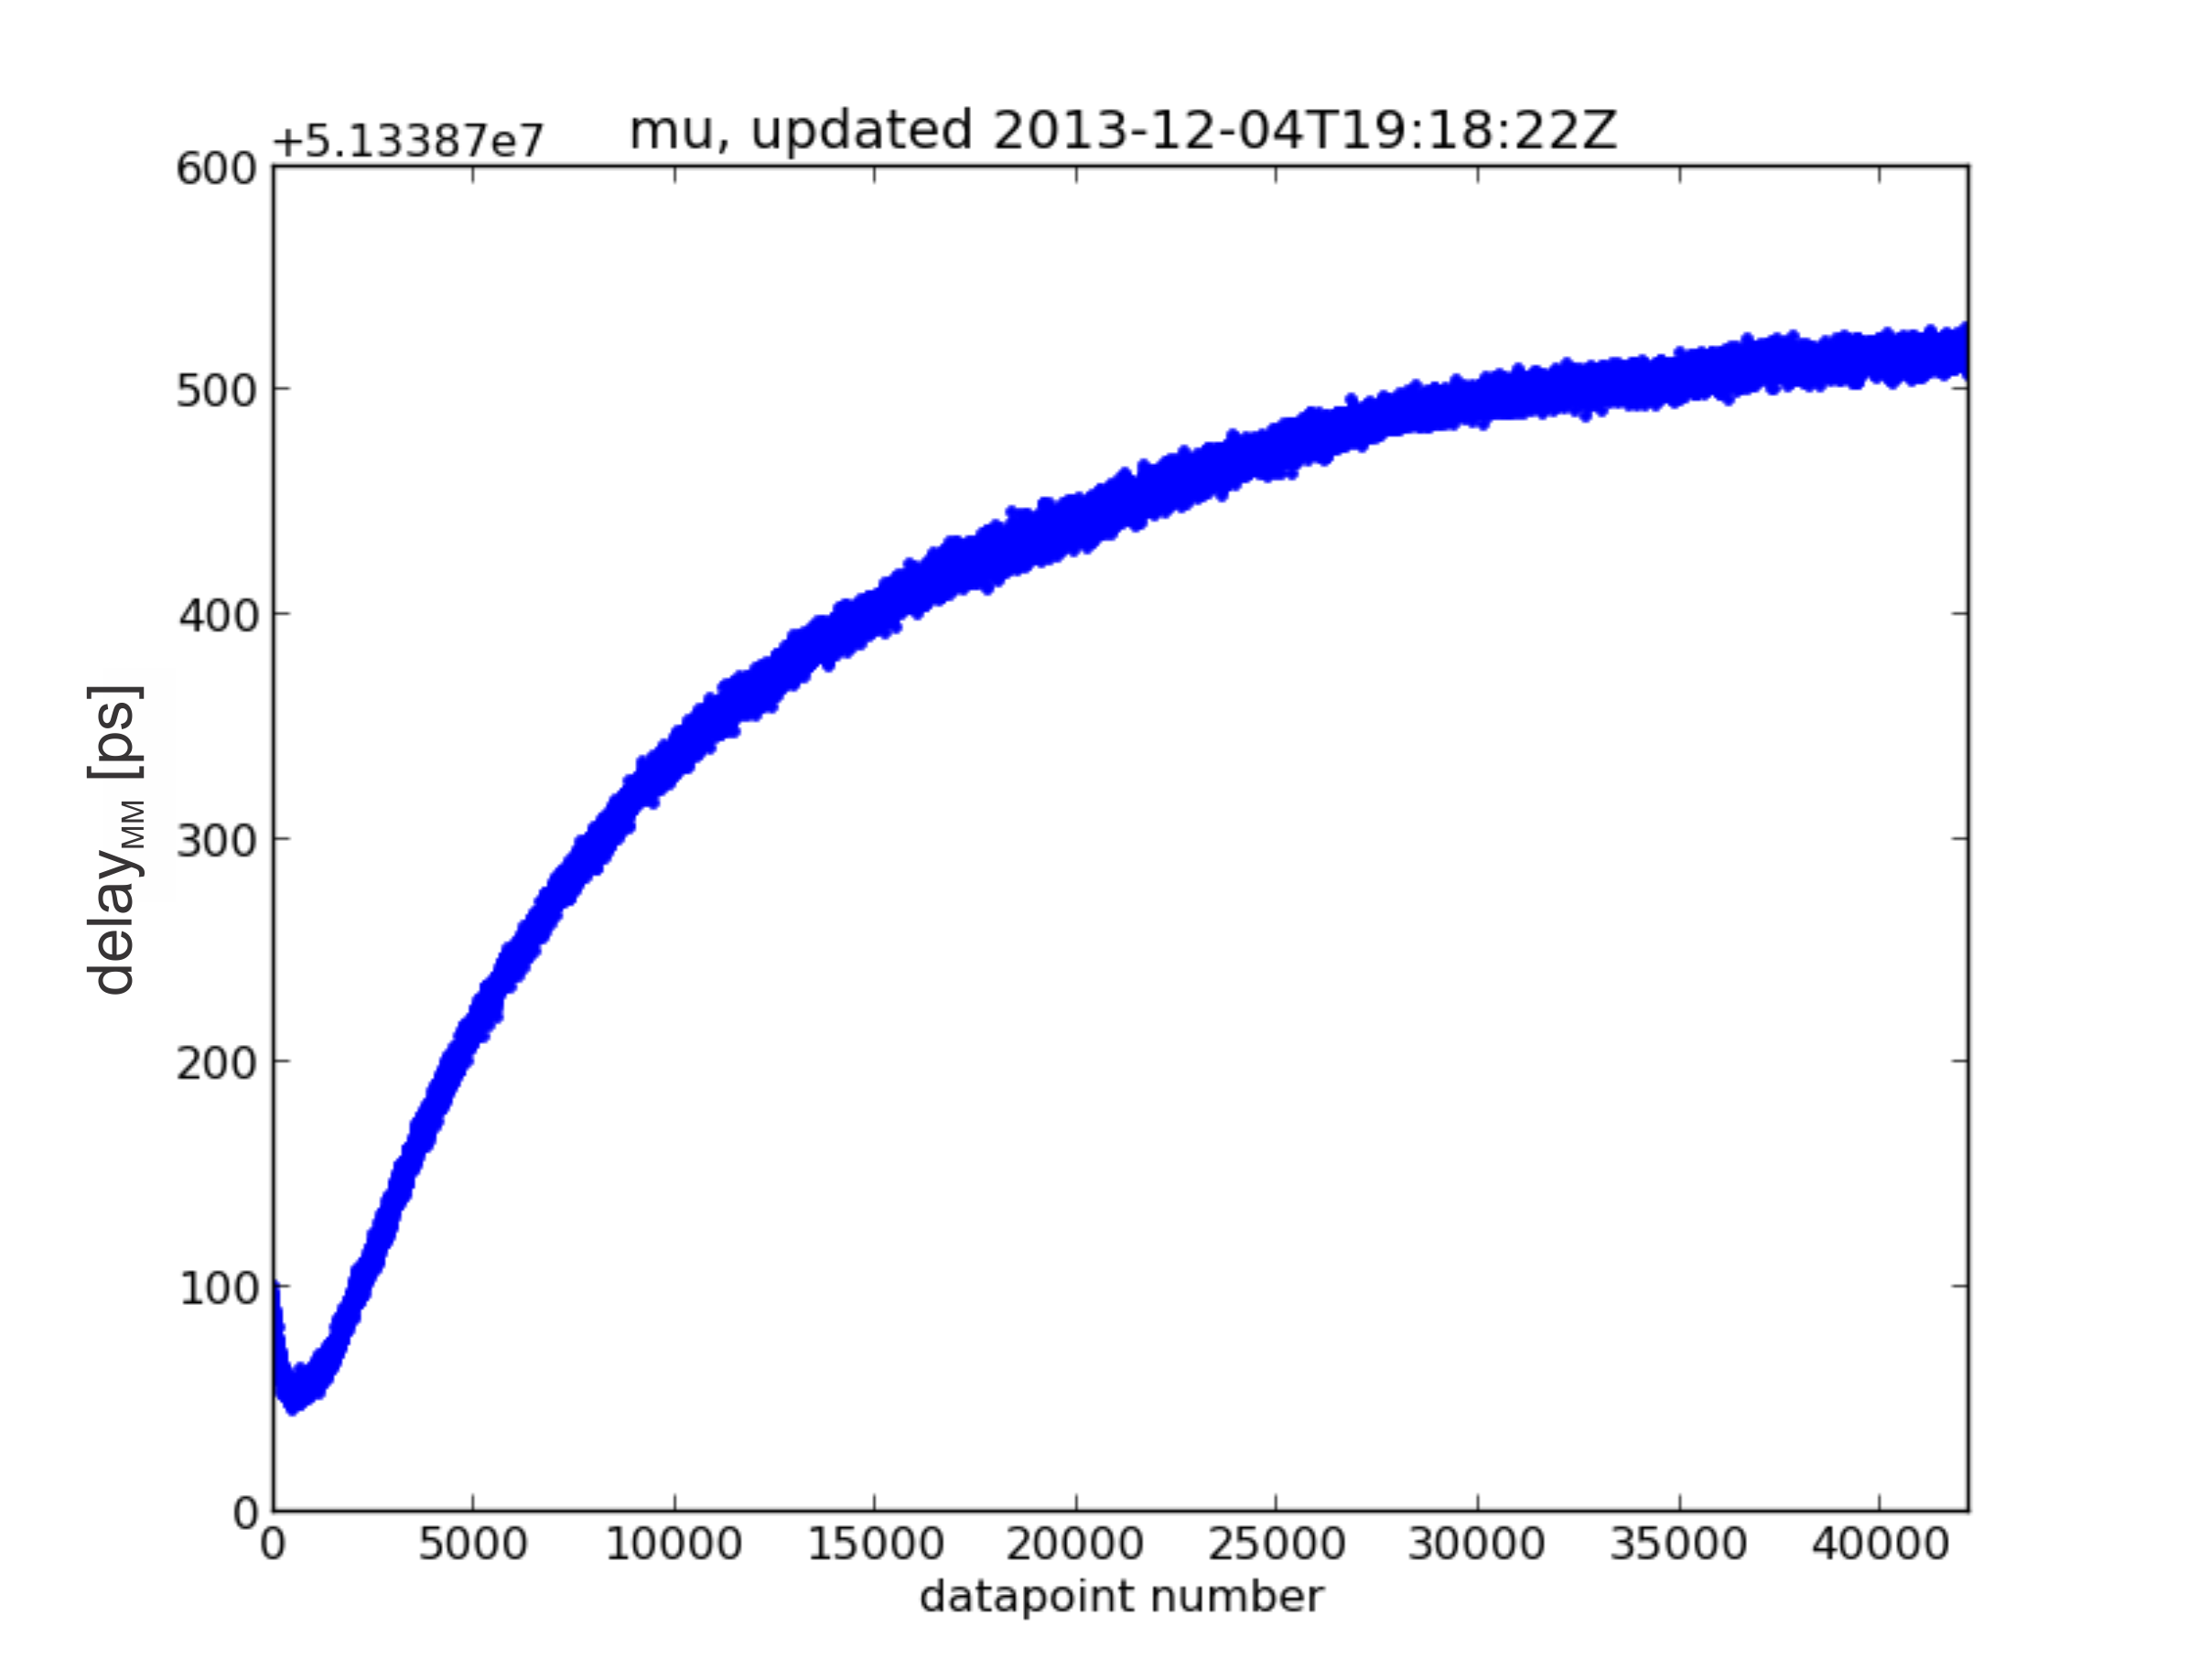
\includegraphics[width=\textwidth]{calibration/rtt_long.png}
\end{minipage}
b)
\begin{minipage}{.5\textwidth}
	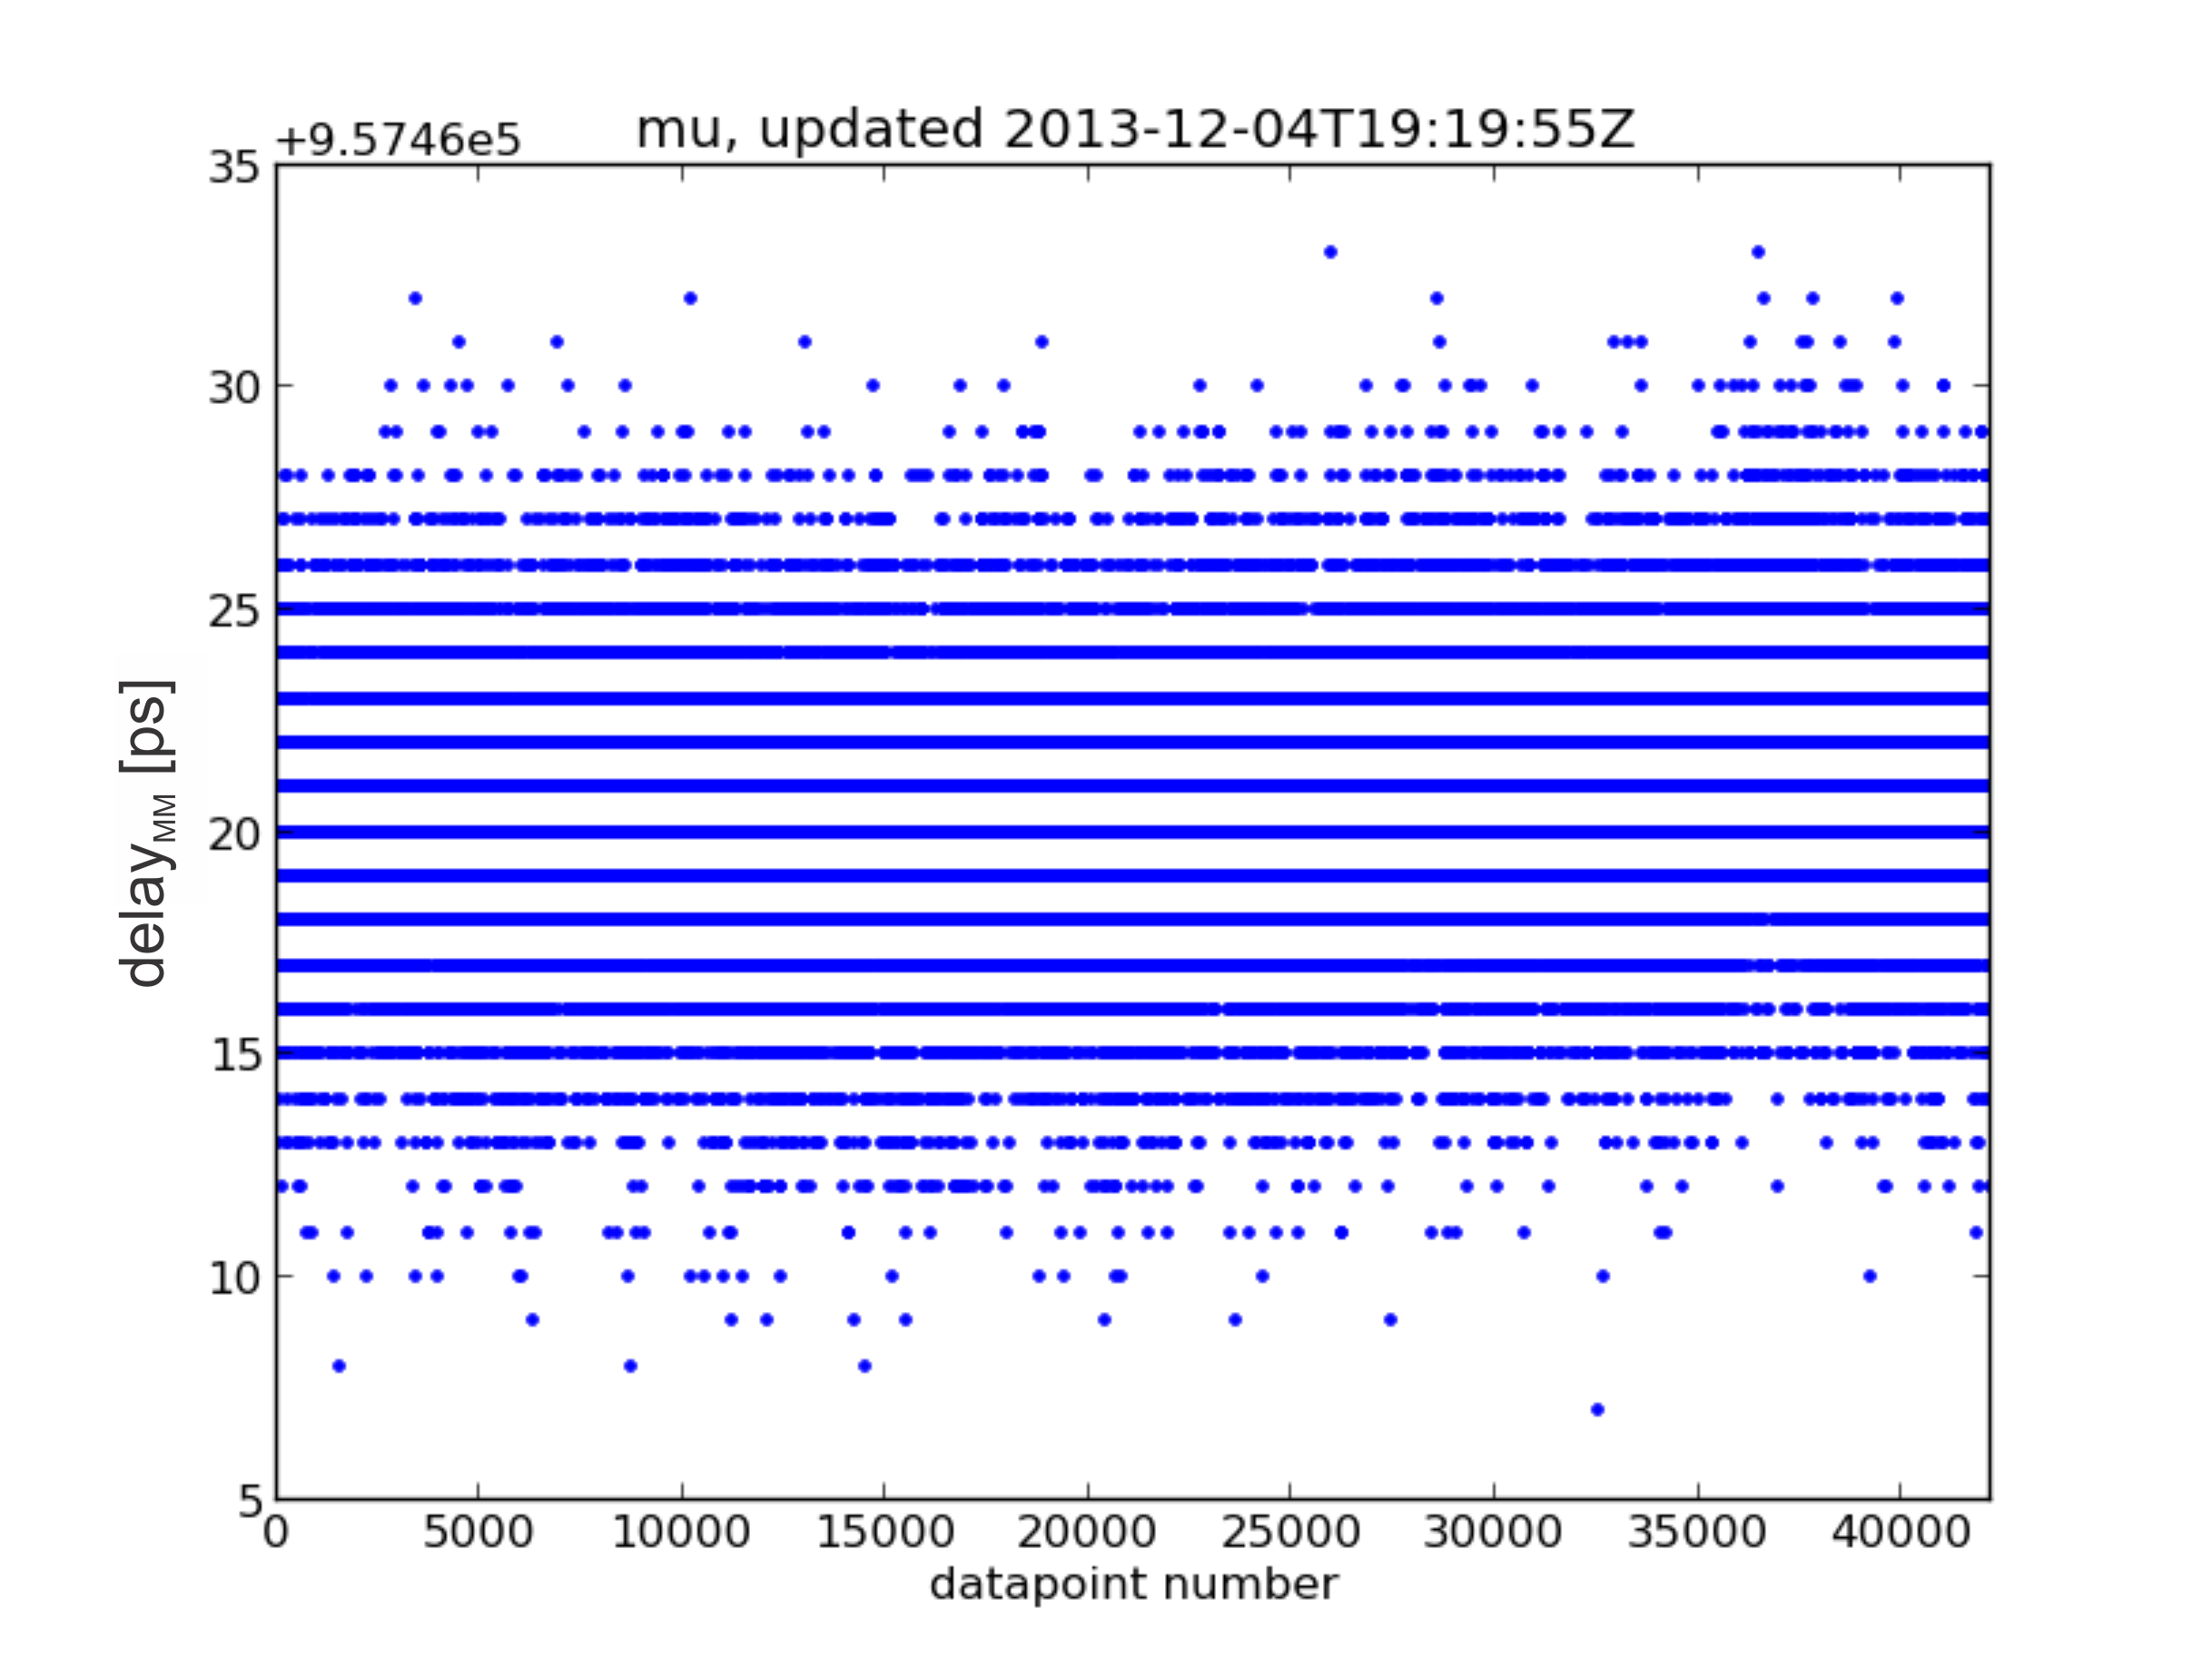
\includegraphics[width=\textwidth]{calibration/rtt_short.png}
\end{minipage}
\caption{$delay_{MM}$ of 5 km (a) and 5 m (b) fiber logged for almost 12 hours using two WR Switches}
\label{fig:errors:deltemp}
\end{figure}
\end{center}

It is noticeable, that the latency of the long fiber (5 km) varies much more
over time (caused by the temperature change) than the latency of the short one.
Table \ref{tab:errors:deltemp} presents the variances calculated for this almost
12-hour data set.
\renewcommand{\arraystretch}{1.2}
\begin{table}[ht]
	\begin{center}
	\begin{tabular}{|r|r|r|}
	\hline
  \emph{fiber len.} & $s^2(\delta)$ [ps$^2$] & $s(\delta)$ [ps]\\
	\hline
	5 m & 7.92 & 2.81\\
	\hline
	5 km & 16273 & 128\\
	\hline
	\end{tabular}
	\caption{Long term uncertainty of $delay_{MM}$ measurement caused by temperature fluctuations}
	\label{tab:errors:deltemp}
	\end{center}
\end{table}
\renewcommand{\arraystretch}{1}

This means, the latency of the long fiber measured once, may not be valid
anymore when used for the calibration procedures few days later - in a different
ambient temperature. There are two conclusions from this fact:
\begin{itemize}
  \item when you want to measure the $\alpha$ parameter of a long fiber, perform
    the latency measurement (section \ref{subsec:refiber}) prior the
    oscilloscope measurements (section \ref{subsec:fiasym});
  \item use a short (few meters) fiber to calibrate a WR Calibrator and all WR
    Devices (sections \ref{sec:procedure:calibrator}, \ref{subsec:devices}),
    then the latency measurement of the short fiber performed only once will be
    accurate enough independently of the ambient temperature.
\end{itemize}


%%%%%%%%%%%%%%%%%%%%%%%%%%%%%%%%%%%%%%%%%%%%%%%%%%%%%%%%%
\subsection{Fiber asymmetry}
\label{subsec:errors:fiasym}

As described in section \ref{subsec:fiasym}, the asymmetry of the fiber is
expressed with the $\alpha$ parameter:
\begin{equation}
	\alpha = \frac{2(skew_{PPS2}-skew_{PPS1})}{\frac{1}{2}\delta - (skew_{PPS2}-skew_{PPS1})}
\end{equation}

\noindent The uncertainty of $\alpha$ depends on:
\begin{itemize}
	\item the uncertainty of the fiber latency estimation ($u^2(\delta)$)
  \item the uncertainty of the 1-PPS skew between the two WR Devices ($u^2(skew_{PPS})$).
\end{itemize}
The former was already addressed in the previous section
(\ref{subsec:errors:filat}). The uncertainty of the 1-PPS skew between two WR
Devices is the measuring instrument uncertainty subtracted from the uncertainty
of 1-PPS skew measurement done with this instrument:
\begin{equation}
  \label{equ:fiasym:skewPPS}
  u^2(skew_{PPS}) = u^2(meas_{PPS}) - u^2(instr.)
\end{equation}

The uncertainty of the instrument (e.g. oscilloscope) can be taken from
its datasheet or measured in the lab. The measurement can be done by feeding
the same signal to both oscilloscope channels (fig.\ref{fig:errors:osc_jitter}).
You can use either a 50 $\Omega$ splitter (fig.\ref{fig:errors:osc_jitter}.1) or
make a daisy-chain connection (fig.\ref{fig:errors:osc_jitter}.2). The
latter requires setting one oscilloscope channel to high impedance and the
other to 50 $\Omega$ termination. The signal fed to an oscilloscope can be taken
from a signal generator (e.g. Agilent 33250A) or it can be also a 62.5MHz clock
output taken from a WR Switch.
\begin{figure}[ht]
	\begin{center}
	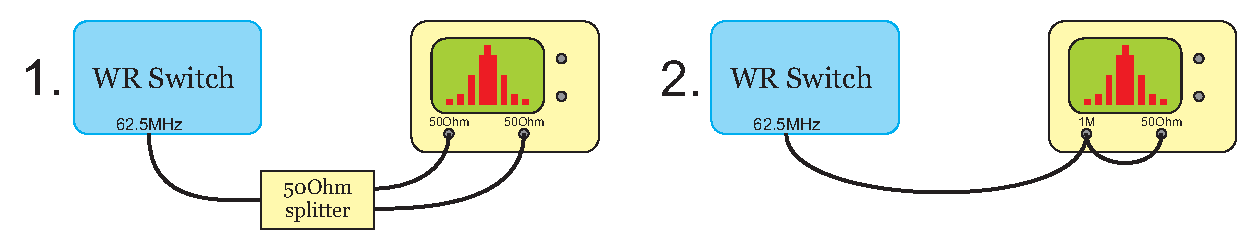
\includegraphics[width=\textwidth]{calibration/oscil_meas.pdf}
	\caption{Measuring internal jitter of an oscilloscope}
	\label{fig:errors:osc_jitter}
	\end{center}
\end{figure}
An example measurement done this way for the \emph{Lecroy Wavepro 7300A}
oscilloscope using a 62.5MHz clock output from a free-running WR Switch is
presented in figure \ref{fig:errors:lecroy_jitter}.
\begin{figure}
	\begin{center}
	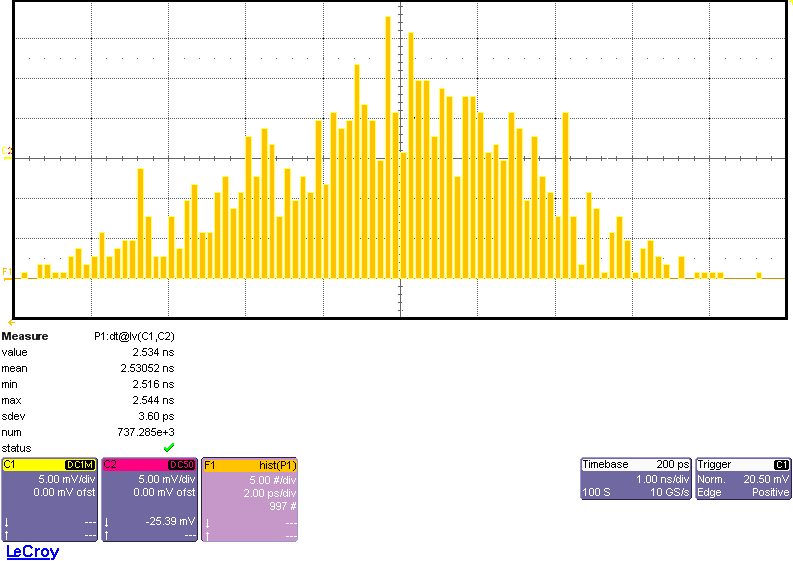
\includegraphics[width=.8\textwidth]{calibration/lecroy_7300_jitter.png}
	\caption{Uncertainty of LeCroy Wavepro 7300A oscilloscope}
	\label{fig:errors:lecroy_jitter}
	\end{center}
\end{figure}
For our considerations the uncertainty of the measuring instrument is:
\begin{align}
	u(instr.) &= 3.6 [ps]\\
	\label{equ:errors:ulecroy}
  u^2(instr.) &= 12.96 [ps^2]
\end{align}

\noindent For comparison, the uncertainty of a \emph{Rhode\&Schwarz RTO1004}
oscilloscope measured the same way is $u^2(instr.) = 30.80 [ps^2]$\\

The next step is to determine the total uncertainty of the 1-PPS skew measurement
($u^2(meas_{PPS})$). It can be done with an oscilloscope by logging the 1-PPS
skew between two synchronized WR Devices. The standard deviation and the
variance can be calculated based on these samples. Parameters measured with the
\emph{Lecroy Wavepro 7300A} for two WR Switches v3.3, two SPECs running the WR
PTP Core v2.1 and the WR Switch with SPEC are presented in table
\ref{tab:errors:ppsjitter}.
\begin{table}[ht]
	\begin{center}
	\begin{tabular}{|l|c|c|}
		\hline
    \emph{devices} & $u(meas_{PPS}) [ps]$ & $u^2(meas_{PPS}) [ps^2]$\\
		\hline
		WR Switch - WR Switch & 9.33 & 87.05\\
		WR Switch - SPEC & 19.37 & 375.20\\
	  SPEC - SPEC & 26.79 & 717.70\\
		\hline
	\end{tabular}
	\end{center}
  \caption{Total jitter of 1-PPS skew measurement}
	\label{tab:errors:ppsjitter}
\end{table}

Using equation \ref{equ:fiasym:skewPPS}, values from \ref{equ:errors:ulecroy}
and table \ref{tab:errors:ppsjitter} the uncertainty of the 1-PPS skew between
two WR Devices can be calculated. The uncertainties for various configurations
are collected in table \ref{tab:errors:skewpps}.
\begin{table}[ht]
  \begin{center}
    \begin{tabular}{|l|c|c|}
      \hline
      \emph{devices} & $u(skew_{PPS}) [ps]$ & $u^2(skew_{PPS}) [ps^2]$\\
      \hline
      WR Switch - WR Switch & 8.61  & 74.09\\
           WR Switch - SPEC & 19.03 & 362.24\\
                SPEC - SPEC & 26.55 & 704.74\\
      \hline
    \end{tabular}
  \end{center}
  \caption{Jitter of 1-PPS skew produced by various WR devices}
  \label{tab:errors:skewpps}
\end{table}

These uncertainties can be used then to calculate the uncertainty of the
$\alpha$ parameter estimated according to step \ref{subsec:fiasym} of the
calibration procedure. To simplify the equations, we introduce a new parameter
$s$ with uncertainty $u^2(s)$:
\begin{align}
	s &= skew_{PPS2} - skew_{PPS1}\\
  u^2(s) &= u^2(skew_{PPS2}) + u^2(skew_{PPS1}) = 2 \cdot u^2(skew_{PPS})
\end{align}

{\bf Note:} If two exactly the same WR Devices (with the same firmware version)
are used for this step of the calibration, then the measured $skew_{PPS1}$ will
be equal to 0 ps. That is because there won't be any asymmetry of the hardware
for a given connection and the asymmetry of a few meters long fiber is
negligible. In such case doing only one measurement of the 1-PPS skew
($skew_{PPS2}$) is enough and estimations $s$, $u^2(s)$ can be simplified:
\begin{align}
	s &= skew_{PPS2}\\
  u^2(s) &= u^2(skew_{PPS})
\end{align}

\noindent By putting parameter $s$ to the $\alpha$ equation we get a new
formula for estimating the uncertainty:
\begin{equation}
	\alpha = \frac{2\cdot s}{\frac{1}{2}\delta - s}
\end{equation}

\noindent The combined standard uncertainty of the $\alpha$ is then estimated as:
\begin{align}
	\label{equ:errors:ualpha}
	u_c^2(\alpha) &= \left( \frac{\partial \alpha}{\partial s} \right)^2 u^2(s) + \left(
	\frac{\partial \alpha}{\partial \delta} \right)^2 u^2(\delta) \nonumber\\
  & = \left( \frac{\delta}{(\frac{1}{2}\delta - s)^2} \right)^2 u^2(skew_{PPS}) + \left(
	\frac{-s}{(\frac{1}{2}\delta - s)^2} \right)^2 u^2(\delta)
\end{align}

Taking a look at the $\left( \frac{\partial \alpha}{\partial s} \right)$ factor,
we can conclude that the influence of the 1-PPS skew uncertainty is smaller when
the latency is greater (fiber is longer):
\begin{equation}
	\lim_{\delta \to \infty} \left( \frac{\partial \alpha}{\partial s} \right) = 0
\end{equation}

As an example we can calculate the combined uncertainty of $\alpha$ using
equation \ref{equ:errors:ualpha} for a 5 km fiber measured with the \emph{LeCroy
Wavepro 7300A} and two WR Switches:
\begin{align}
  &\delta = 50421913 [ps] \hspace{1cm} s = 3243 [ps]\nonumber \\
  &u^2(\delta) = 14.4 [ps^2] \hspace{1cm} u^2(skew_{PPS}) = 74.09 [ps^2] \nonumber \\
	\label{equ:errors:alpha}
	\alpha &= 2.573e-4 \\
	\label{equ:errors:unc_alpha}
  u_c^2(\alpha) &= 4.665e-13\\
	\label{equ:errors:stdev_alpha}
  u_c(\alpha) &= 0.0068e-4
\end{align}

The uncertainty of $\alpha$ may cause about \emph{9 ps} of uncompensated
asymmetry in a 5km link. It can be calculated by subtracting the WR PTP
$delay_{MS}$ estimations for the measured $\alpha$ (equation
\ref{equ:errors:alpha}) and for $\alpha$ distorted by its standard deviation:
\begin{equation}
	error = delay_{MS}(\alpha \pm u_c(\alpha)) - delay_{MS}(\alpha) \approx 9 [ps]
\end{equation}

%%%%%%%%%%%%%%%%%%%%%%%%%%%%%%%%%%%%%%%%%%%%%%%%%%%%%%%%%
\subsection{Calibrator pre-calibration}
The parameters of a WR Calibrator determined in the calibration procedure depend
on two experimental values:
\begin{itemize}
	\item round trip delay $delay_{MM}$
	\item fiber latency $\delta$
\end{itemize}

The combined standard uncertainties of a transmission and reception delay are the
same and can be estimated in a similar way as in previous sections:
\begin{align}
	u_c^2(\Delta_{TX}) &= u_c^2(\Delta_{RX}) \\
	u_c^2(\Delta_{TX}) &= \left( \frac{\partial \Delta_{TX}}{\partial delay_{MM}}
	\right)^2 u^2(delay_{MM}) + \left( \frac{\partial \Delta_{TX}}{\partial
	\delta} \right)^2 u^2(\delta) \nonumber\\
	&= \frac{1}{16} u^2(delay_{MM}) + \frac{1}{16} u^2(\delta)
\end{align}

As an example we can calculate the combined uncertainty of $\Delta_{TX}$ when
port \emph{1} of the WR Switch is selected to be a WR Calibrator and the calibration is
done with the 5m fiber used in the previous steps. To evaluate the worst case, the
uncertainties for single sample measurements (not means) are used here
($s^2(del_{MM})$ from table \ref{tab:errors:dmm} and $u^2_c(\delta_1)$ from
equation \ref{equ:errors:f1lat}):
\begin{align}
	u_c^2(\Delta_{TX}) &= \frac{1}{16} \cdot 5.38 + \frac{1}{16} \cdot 17.5  =
  1.43 [ps^2]\\
	u_c(\Delta_{TX}) &= 1.20 [ps]
\end{align}

%%%%%%%%%%%%%%%%%%%%%%%%%%%%%%%%%%%%%%%%%%%%%%%%%%%%%%%%%
\subsection{WR Device calibration}
The last step of the calibration procedure depends on all the previous stages.
First, we should estimate the uncertainty of the coarse (average) transmission
and reception delays of a WR Device. Rewriting equation
\ref{equ:devices:coarsedtxrx} and omitting the bitslide value gives us equation
\ref{equ:errors:devices:dtxrx} which is used for the uncertainty
estimation (\ref{equ:errors:devices:udtxrx}). The fixed delays of the WR
Calibrator are represented by symbols $\Delta_{TXC}$ and $\Delta_{RXC}$.
\begin{align}
	\label{equ:errors:devices:dtxrx}
	\Delta'_{TXS} &= \Delta'_{RXS} = \frac{1}{2}(delay_{MM} - \Delta_{TXC} -
	\Delta_{RXC} - \delta)\\
	\label{equ:errors:devices:udtxrx}
	u^2(\Delta'_{TXS}) &= \left( \frac{\partial \Delta'_{TXS}}{\partial delay_{MM}} \right)^2 u^2(delay_{MM}) +
	2 \cdot \left( \frac{\partial \Delta'_{TXS}}{\partial \Delta_{TXC}} \right)^2 u^2(\Delta_{TXC}) +
	\left( \frac{\partial \Delta'_{TXS}}{\partial \delta} \right)^2 u^2(\delta) \nonumber\\
	&= \frac{1}{4} u^2(delay_{MM}) + \frac{1}{2} u^2(\Delta_{TXC}) + \frac{1}{4} u^2(\delta)
\end{align}

For the case when the WR Switch is the calibrator, the WRPC running on a SPEC is
the WR Device under calibration and the connection is made with a short fiber,
the uncertainty of the coarse fixed delay is:
\begin{align}
	u^2(\Delta'_{TXS}) &= u^2(\Delta'_{RXS}) = \frac{1}{4} \cdot 17.58 +
  \frac{1}{2} \cdot 1.43 + \frac{1}{4} \cdot 17.5 = 9.49 [ps^2]\\
	u(\Delta'_{TXS}) &= u(\Delta'_{RXS}) = 3.08 [ps]
\end{align}\\

The second part of the WR Device calibration uses the 1-PPS skew readout from
the oscilloscope as the correction value $\beta$ to compensate fixed delay
asymmetry. The uncertainty of the estimation of $\beta$ is then the sum of two
factors: the uncertainty of the 1-PPS skew measurement (the same as in
\ref{subsec:errors:fiasym}) and the uncertainty of the one way delay
($delay_{MS}$) estimation in the WR PTP software:
\begin{equation}
	\label{equ:errors:ubeta}
	u^2(\beta) = u^2(skew_{PPS}) + u^2(delay_{MS})
\end{equation}

\noindent Knowing the formula used by the WR PTP software for estimating $delay_{MS}$:
\begin{equation}
	delay_{MS} = \frac{1+\alpha}{2+\alpha}(delay_{MM} - \Delta) + \Delta_{TXM} +
	\Delta_{RXS}
\end{equation}
we can calculate the uncertainty of this estimation:
\begin{align}
	u^2(delay_{MS}) &= \left( \frac{\partial delay_{MS}}{\partial \alpha} \right)^2 u^2(\alpha) + 
	\left( \frac{\partial delay_{MS}}{\partial delay_{MM}}\right)^2 u^2(delay_{MM}) \nonumber\\
	&+ \left( \frac{\partial delay_{MS}}{\partial \Delta}\right)^2 u^2(\Delta) +
	\left( \frac{\partial delay_{MS}}{\partial \Delta_{TXC}}\right)^2 u^2(\Delta_{TXC}) \nonumber\\
	&+ \left( \frac{\partial delay_{MS}}{\partial \Delta_{RXS}}\right)^2 u^2(\Delta'_{RXS})
\end{align}

\noindent All the necessary uncertainties but $u^2(\Delta)$ were calculated in previous
sections. However, $\Delta$ is the sum of the coarse fixed delays of the Master
(Calibrator) and the Slave, so:
\begin{align}
	\label{equ:errors:ubigd}
	u^2(\Delta) &= 2\cdot u^2(\Delta_{TXC}) + 2\cdot u^2(\Delta'_{RXS}) \noindent\\
              &= 2 \cdot 1.43 + 2 \cdot 9.49 = 21.84 [ps^2]
\end{align}

Table \ref{tab:errors:wrdev} presents the values from the SPEC calibration (the
WR Switch was the Calibrator) and collects together other uncertainties
calculated in previous sections. Please note that the transmission and reception
fixed delays are not equal because of the bitslide. They could have been
omitted earlier, but now have to be taken into account for $\Delta$ calculation.
\begin{table}[ht]
	\begin{center}
	\mbox{a)
	\begin{tabular}{|c|c|c|c|c|c|}
		\hline
		$delay_{MM}$ & $\Delta_{TXC}$ & $\Delta_{RXC}$ & $\Delta_{TXS}$ & $\Delta_{RXS}$ & $\alpha$\\
		\hline \hline
		838152 & 225030 & 228230 & 164261 & 170661 & 2.573e-4\\
		\hline
  \end{tabular}}\\

	\vspace{6pt}

	\mbox{b)
	\begin{tabular}{|c|c|c|c|c|}
		\hline
    $u^2(\alpha)$ & $u^2(delay_{MM}) [ps^2]$ & $u^2(\Delta) [ps^2]$ & $u^2(\Delta_{TXC}) [ps^2]$ & $u^2(\Delta'_{RXS}) [ps^2]$\\
		\hline \hline
		4.665e-13 & 17.58 & 21.84 & 1.43 & 9.49\\
		\hline
  \end{tabular}}
	\end{center}
	\caption{Example of SPEC calibration values when being calibrated to a WR Switch
		(a) and uncertainties calculated in previous sections (b)}
	\label{tab:errors:wrdev}
\end{table}

Using these values we can calculate the uncertainty of the estimation of
$delay_{MS}$ (\ref{equ:errors:udms}).
\begin{align}
	\label{equ:errors:udms}
	u^2(delay_{MS}) &= \left( \frac{delay_{MM}-\Delta}{(2+\alpha)^2} \right)^2 u^2(\alpha) +
	\left( \frac{1+\alpha}{2+\alpha} \right)^2 u^2(delay_{MM}) \nonumber\\
	&+ \left( -\frac{1+\alpha}{2+\alpha} \right)^2 u^2(\Delta) + u^2(\Delta_{TXC})
	+ u^2(\Delta'_{RXS})\\
  u^2(delay_{MS}) &= 20.78 [ps^2]\\
	u(delay_{MS}) &= 4.56 [ps]
\end{align}

Taking the uncertainty of the 1-PPS skew produced by the SPEC and the WR Switch
(table \ref{tab:errors:skewpps}) and comparing it to the uncertainty of the
estimation of $delay_{MS}$ and the uncertainty of the measuring instrument
(equation \ref{equ:errors:ulecroy}) we can conclude that almost all of the
uncertainty comes from the jitter of the 1-PPS output from the SPEC:
\begin{align}
  u^2(\beta) &= u^2(skew_{PPS}) + u^2(delay_{MS}) \approx u^2(skew_{PPS}) \approx
  362 [ps^2]\\
	u(\beta) &\approx 19 [ps]
\end{align}


\newpage
\bibliographystyle{unsrt}
\bibliography{references}

\end{document}
